\documentclass[10pt, reqno]{exam}
\usepackage[utf8]{inputenc}
\usepackage{amsthm}
\usepackage{libertine}
\usepackage[margin=0.5in, includefoot]{geometry}
\usepackage{amsmath,amssymb}
\usepackage{multicol}
\usepackage[shortlabels]{enumitem}
\usepackage{cancel}
\usepackage{listings}
\usepackage{tikz}
\usepackage{float}
\usepackage{mathtools}
\usepackage{wrapfig, lipsum}
\usepackage{chemfig}
\usepackage{chemmacros}
\usepackage{chemformula}
\usepackage{empheq}
\usepackage{caption}
\usepackage{subcaption}
\usepackage[normalem]{ulem}
\usepackage{graphicx}
\usepackage{bm}
\usepackage{accents}
\usepackage[T1]{fontenc}
\usepackage[font=small,labelfont=bf,tableposition=top]{caption}
\usepackage{siunitx}
\usepackage{minted}
\usepackage{etoolbox}
\usepackage{multirow}
\usepackage[version=4]{mhchem}
\usepackage{pgfplots}
\usepackage{svg}
\usepackage{upgreek}
\usepackage{longtable}
\usepackage{graphics}
\usepackage[colorlinks=true,allcolors=blue]{hyperref}
\usepackage{parskip}

\pgfplotsset{compat=1.18}

\AtBeginEnvironment{minted}{
    \fontsize{8}{10}\selectfont}
\newcommand{\fahrenheit}{^\circ{F}}
\newcommand*\widefbox[1]{\fbox{\hspace{2em}#1\hspace{2em}}}
\newcommand{\msout}[1]{
    \text{\sout{$#1$}}
}
\usetikzlibrary{shapes}
\DeclareSIUnit\year{y}
\sisetup{group-digits = integer, group-minimum-digits = 3, group-separator = {,}}
\newcommand{\class}{Dr. Shao's Research Group}
\newcommand{\examnum}{eSRIM Code Walkthrough}
\newcommand{\examdate}{Feburary 17\textsuperscript{th}, 2024}
\newcommand{\timelimit}{}
\newcommand{\laplace}{\mathcal{L}}

\begin{document}

\begingroup
\hbadness=10000
\noindent 
\begin{tabular*}{\textwidth}{l @{\extracolsep{\fill}} r @{\extracolsep{4pt}} l}
  \textbf{\class} & \textbf{Name:} & \textit{Nathaniel Thomas}\\ %Your name here instead, obviously 
  \textbf{\examnum}  && \\
  \textbf{\examdate} && \\
\end{tabular*}\\


\noindent\hrule width \textwidth height 2pt

\tableofcontents

\pagebreak

\listoffigures

\listoftables

\pagebreak

\section{Introduction}

This document contains a walkthrough of the eSRIM code written by Dr. Lin Shao. In addition, it also contains notes on QuickBASIC, the language that the original code is written in, as well as a plan for conversion of the code to a more performant language, C++. \par



This document goes through the QuickBASIC code (dubbed eSRIM) written by Dr. Shao in line-by-line detail, explaining the purpose of each line of code in as much detail as possible. While some familiarization with code is required, Section \ref{sec:syntax} contains tables with the important keywords and reserved characters in QuickBASIC, allowing one to rapidly search for syntax that they are unfamiliar with in QuickBASIC, should they be unable to acertain the purpose of the code through context. \par

QuickBASIC is a very readable language that is reasonably performant, due to the conversion of the code directly to machine code (the fastest form of code). Other programming languages (such as Python) instead use an "\href{https://en.wikipedia.org/wiki/Interpreter_(computing)}{interpreter}", which is a program that reads one line of code at a time and executes. Due to the nature of this type of programming language, Python is often not very performant. On the other hand, QuickBASIC is a compiled language, meaning that it uses a "\href{https://en.wikipedia.org/wiki/Compiler}{compiler}" to convert the source code directly to machine language for the comptuer's Central Processing Unit (CPU) to execute directly. This is the most performant type of programming language. \par

Despite the performance benefit of being a compiled language, QuickBASIC is still far from being the most performant programming language. Several techniques can be used to further optimize eSRIM. For example, "\href{https://en.wikipedia.org/wiki/Multithreading_(computer_architecture)}{multi-threading}" can be used to simulate many particle collisions simultaneously. Compilers can also be used to optimize code directly using several advanced techniques. Some of these techniques include "\href{https://en.wikipedia.org/wiki/Loop_unrolling}{loop-unrolling}" or "\href{https://en.wikipedia.org/wiki/Inline_expansion}{function in-lining}". The art of low-level program optimization is a very complex and extensive field that can lead to order-of-magnitude improvements in code execution speed. However, these techniques are not utilized in QuickBASIC compilers to the same extent as they are in compilers for C++ such as \href{https://en.wikipedia.org/wiki/GNU_Compiler_Collection}{g++} or \href{https://en.wikipedia.org/wiki/Clang}{clang}. \par

Maximizing performance in this type of simulation is important, as this type of simulation (\href{https://en.wikipedia.org/wiki/Monte_Carlo_method}{Monte-Carlo Method}) requires extensive generation of data. In the case of eSRIM, as many as 1000 simulations or more are needed to generate useful data. While the QuickBASIC eSRIM code can simulate several electron collisions (which is more computationally intensive than ion collisions) per second using the flying distance grouping optimization method (discussed later), this can still result in simulations taking several minutes to complete. By rewriting the code in a more optimized form, it is projected that the same simulations can take mere seconds. \par

\clearpage

\section{Notes on Syntax}
\label{sec:syntax}

This section contains two tables which can be used to understand how QuickBASIC syntax works. Table \ref{tbl:keywords} contains all of the keywords used in QuickBASIC in alphabetical order. This table can be used to understand how each keyword is used in QuickBASIC. \par

Table \ref{tbl:reserved characters} contains all of the reserved characters in QuickBASIC. These are special characters that QuickBASIC recognizes and performs special actions when it encounters them. For example, a single quote "'" is treated as a comment, and any text following a single quote on the same line is treated as a comment, meaning that the content of the comment is not considered code, and therefore the contents of a comment does not affect the functionality of the code. This is useful in describing the functionality of code. \par

\subsection{Keywords}

There are several reserved "keywords" in QuickBASIC which carry special meaning to the QuickBASIC compiler. Table \ref{tbl:keywords} contains a largely comprehensive list of all of these keywords, as well as their purpose: \par

% Generated using ChatGPT 3.5, prompt: 
% I am tabulating all of the keywords in QuickBASIC, along with their type (Function, Operator, etc.), use ( varA AND varB, for example), and purpose. This is a template with the ABS keyword.

% \begin{table}[h]
%     \centering
%     \begin{tabular}{|c|c|c|c|c|}
%         \hline
%         Keyword & Type & Use  & Purpose  \\
%         \hline
%         ABS & Function & ABS(x), x is a SINGLE, DOUBLE, or INT & Calculate absolute value of a number \\
%         \hline
%     \end{tabular}
%     \caption{Comprehensive list of all QuickBASIC Keywords}
%     \label{tbl:keywords}
% \end{table}

% Please provide a complete version of this table for all  QuickBASIC keywords.

{
\footnotesize
\begin{longtable}{|c|c|c|c|}
    \caption{Comprehensive list of all QuickBASIC Keywords}
    \label{tbl:keywords} \\
    \hline
    Keyword & Type & Use & Purpose \\
    \hline
    ABS & Function & ABS(x) & Calculate absolute value of a number \\
    ACCESS & Statement & ACCESS mode, path & Set or return the access mode of a file \\
    AND & Operator & varA AND varB & Logical AND operation \\
    ANY & Operator & varA ANY varB & Bitwise OR operation \\
    APPEND & Statement & APPEND mode, path & Open a file for appending data \\
    AS & Keyword & DIM var AS type & Declare a variable with a specific data type \\
    ASC & Function & ASC(string) & Return ASCII code of the first character in a string \\
    ATN & Function & ATN(x) & Return arctangent of a number \\
    BASE & Statement & BASE value & Set or return the default base for numeric input and output \\
    BEEP & Statement & BEEP & Produce a beep sound \\
    BLOAD & Statement & BLOAD "filename", address & Load binary data from a file into memory \\
    BSAVE & Statement & BSAVE "filename", address, length & Save binary data from memory to a file \\
    BYVAL & Keyword & BYVAL parameter & Pass a parameter by value in a procedure \\
    CALL & Statement & CALL subroutine & Call a subroutine or function \\
    CALLS & Function & CALLS & Return number of subroutine or function calls \\
    CASE & Keyword & SELECT CASE expression & Define a case in a SELECT CASE structure \\
    CHAIN & Statement & CHAIN "filename" & Start execution of another program file \\
    CHDIR & Statement & CHDIR "path" & Change current directory \\
    CHR\$ & Function & CHR\$(code) & Return character associated with ASCII code \\
    CIRCLE & Statement & CIRCLE (x, y), radius & Draw a circle on the screen \\
    CLEAR & Statement & CLEAR & Clear all variable values \\
    CLNG & Function & CLNG(expression) & Convert expression to a long integer \\
    CLOSE & Statement & CLOSE [fileNumber] & Close an open file \\
    CLS & Statement & CLS & Clear the screen \\
    COLOR & Statement & COLOR foreground, background & Set text and background colors \\
    COMMON & Statement & COMMON [sharedVariable] & Declare shared variables \\
    CONST & Statement & CONST constantName = value & Define a constant \\
    COS & Function & COS(angle) & Return cosine of an angle \\
    CSRLIN & Function & CSRLIN & Return current cursor line position \\
    CVD & Function & CVD(string) & Convert string to a date value \\
    CVDMBF & Function & CVDMBF(string) & Convert string to a date value using the default date format \\
    CVI & Function & CVI(string) & Convert string to an integer value \\
    CVL & Function & CVL(string) & Convert string to a long integer value \\
    CVS & Function & CVS(string) & Convert string to a single-precision floating-point value \\
    DATA & Statement & DATA value1, value2, ... & Define data for READ statement \\
    DATE\$ & Function & DATE\$ & Return current date \\
    DECLARE & Statement & DECLARE subName [LIB "libraryName"] & Declare external subroutines or functions \\
    DEF FN & Statement & DEF FN functionName (parameters) = expression & Define a user-defined function \\
    DEF SEG & Statement & DEF SEG = segmentAddress & Set default segment for memory access \\
    DEFDBL & Statement & DEFDBL variableList & Declare double-precision variables by default \\
    DEFINT & Statement & DEFINT variableList & Declare integer variables by default \\
    DEFLNG & Statement & DEFLNG variableList & Declare long integer variables by default \\
    DEFSNG & Statement & DEFSNG variableList & Declare single-precision variables by default \\
    DEFSTR & Statement & DEFSTR variableList & Declare string variables by default \\
    DEFVAR & Statement & DEFVAR variableList & Declare variables with specific data types by default \\
    DELETE & Statement & DELETE & Delete a line in a program \\
    DIM & Statement & DIM array(dimensions) & Declare array variables \\
    DO & Statement & DO & Start a DO...LOOP loop \\
    DOUBLE & Type & DOUBLE & Double-precision floating-point data type \\
    DRAW & Statement & DRAW "action" & Draw graphics primitives \\
    DSKO\$ & Function & DSKO\$(drive) & Return description of disk \\
    DSKI\$ & Function & DSKI\$(drive) & Return information about disk \\
    ELSE & Keyword & IF condition THEN statement ELSE statement & Execute if condition is false \\
    ELSEIF & Keyword & IF condition THEN statement ELSEIF condition THEN statement & Execute if previous condition is false and current condition is true \\
    END & Statement & END & Terminate program execution \\
    END FUNCTION & Statement & END FUNCTION & End a function definition \\
    END IF & Statement & END IF & End an IF...THEN...ELSE block \\
    END SELECT & Statement & END SELECT & End a SELECT CASE block \\
    END SUB & Statement & END SUB & End a subroutine definition \\
    END TYPE & Statement & END TYPE & End a user-defined type definition \\
    END WHILE & Statement & END WHILE & End a WHILE...WEND loop \\
    ENVIRON\$ & Function & ENVIRON\$(name) & Return value of an environment variable \\
    EOF & Function & EOF(fileNumber) & Test for end of file \\
    ERASE & Statement & ERASE array & Delete array variables \\
    ERDEV & Function & ERDEV & Return error device number \\
    ERDEV\$ & Function & ERDEV\$ & Return error device name \\
    ERL & Function & ERL & Return line number of last error \\
    ERR & Function & ERR & Return error number \\
    ERROR\$ & Function & ERROR\$ & Return error message \\
    EXIT & Statement & EXIT DO & Exit a DO...LOOP loop \\
    EXP & Function & EXP(x) & Return exponential value of a number \\
    FIELD & Statement & FIELD [fileNumber], fieldNumber AS fieldDefinition & Define random-access file records \\
    FILES\$ & Function & FILES\$ & Return files in the current directory \\
    FILL & Statement & FILL & Fill graphics screen with a color \\
    FIX & Function & FIX(number) & Return integer part of a number \\
    FNEND & Statement & FNEND & End a user-defined function \\
    FOR & Statement & FOR counter = start TO end [STEP step] & Start a FOR...NEXT loop \\
    FORMAT\$ & Function & FORMAT\$(expression, format) & Format a numeric value \\
    FRAME & Statement & FRAME & Draw a frame around the graphics screen \\
    FREEFILE & Function & FREEFILE & Return a free file number \\
    FREQUENCY & Function & FREQUENCY & Return timer frequency \\
    FUNCTION & Statement & FUNCTION functionName (parameters) & Define a function \\
    GET & Statement & GET [fileNumber, ]recordNumber & Read a record from a random-access file \\
    GOSUB & Statement & GOSUB lineLabel & Call a subroutine \\
    GOTO & Statement & GOTO lineLabel & Unconditional jump to a line label \\
    HEX\$ & Function & HEX\$(number) & Return hexadecimal representation of a number \\
    IF & Statement & IF condition THEN statement & Execute if condition is true \\
    IMP & Operator & varA IMP varB & Logical implication \\
    INKEY\$ & Function & INKEY\$ & Check for a key press \\
    INP & Function & INP(port) & Read from an I/O port \\
    INPUT & Statement & INPUT prompt; variable & Prompt user for input \\
    INPUT\$ & Function & INPUT\$(prompt) & Prompt user for input and return string \\
    INPUT\# & Statement & INPUT\# fileNumber, variable & Read from an input file \\
    INSTR & Function & INSTR([start, ]string1, string2) & Return position of one string within another \\
    INT & Function & INT(number) & Return integer part of a number \\
    IRQ & Function & IRQ(number) & Return interrupt request status \\
    KILL & Statement & KILL "filename" & Delete a file \\
    LEFT\$ & Function & LEFT\$(string, count) & Return leftmost characters of a string \\
    LEN & Function & LEN(string) & Return length of a string \\
    LET & Statement & LET variable = expression & Assign a value to a variable \\
    LINE & Statement & LINE (x1, y1)-(x2, y2) & Draw a line on the screen \\
    LINE INPUT & Statement & LINE INPUT prompt; variable & Prompt user for input and read a line \\
    LINE INPUT\# & Statement & LINE INPUT\# fileNumber, variable & Read a line from an input file \\
    LOAD & Statement & LOAD "filename" & Load and run a program \\
    LOCATE & Statement & LOCATE row, column & Move cursor to specified position \\
    LOCK & Statement & LOCK [recordNumber] & Lock a record in a random-access file \\
    LOF & Function & LOF(fileNumber) & Return length of an open file \\
    LOG & Function & LOG(number) & Return natural logarithm of a number \\
    LONG & Type & LONG & Long integer data type \\
    LPOS & Function & LPOS & Return current cursor column position \\
    LPRINT & Statement & LPRINT expression & Print to the printer \\
    LSET & Statement & LSET variable = string & Assign a string to a variable \\
    LTRIM\$ & Function & LTRIM\$(string) & Return string with leading spaces removed \\
    MID\$ & Function & MID\$(string, start[, length]) & Return a substring of a string \\
    MKD\$ & Function & MKD\$(dateValue) & Convert date value to string \\
    MKDIR & Statement & MKDIR "path" & Create a directory \\
    MKI\$ & Function & MKI\$(integerValue) & Convert integer value to string \\
    MKL & Function & MKL(longValue) & Convert long integer value to string \\
    MKS\$ & Function & MKS\$(singleValue) & Convert single-precision value to string \\
    MOD & Operator & varA MOD varB & Modulus (remainder) operation \\
    NAME & Statement & NAME "oldName" AS "newName" & Rename a file or directory \\
    NEW & Statement & NEW & Clear memory and reset program execution \\
    NEXT & Statement & NEXT counter & Increment counter in a FOR...NEXT loop \\
    NOT & Operator & NOT expression & Logical negation \\
    OCT\$ & Function & OCT\$(number) & Return octal representation of a number \\
    ON & Statement & ON expression GOSUB lineLabel & Define a line label for GOSUB or GOTO \\
    OPEN & Statement & OPEN mode, fileNumber, "filename" & Open a file for input, output, or append \\
    OPTION & Statement & OPTION BASE number & Set the base index for array dimensions \\
    OR & Operator & varA OR varB & Logical OR operation \\
    OUT & Statement & OUT port, value & Write to an I/O port \\
    OUTPUT & Statement & OUTPUT & Switch output to the screen \\
    OVERLAY & Statement & OVERLAY "filename" & Overlay the current program with another program \\
    PAINT & Statement & PAINT (x, y), fillColor, borderColor & Fill an enclosed area with color \\
    PEN & Statement & PEN color & Set pen color for graphics drawing \\
    PLAY & Statement & PLAY "notes" & Play music notes \\
    POINT & Function & POINT(x, y) & Return color of a point on the screen \\
    POKE & Statement & POKE address, value & Write a value to a memory address \\
    POS & Function & POS & Return current cursor position \\
    PRINT & Statement & PRINT expression & Print to the screen \\
    PRINT USING & Statement & PRINT USING format; expression & Print using a specified format \\
    PSET & Statement & PSET (x, y), color & Set a pixel to a specified color \\
    PUT & Statement & PUT [fileNumber, ]recordNumber & Write a record to a random-access file \\
    RANDOMIZE & Statement & RANDOMIZE [seed] & Initialize random number generator \\
    READ & Statement & READ variableList & Read data from a DATA statement \\
    REDIM & Statement & REDIM array(dimensions) & Redimension an array \\
    REM & Statement & REM comment & Add a remark or comment to the code \\
    RESTORE & Statement & RESTORE [lineLabel] & Reset data pointer for READ statement \\
    RESUME & Statement & RESUME [lineLabel] & Resume execution after an error \\
    RETURN & Statement & RETURN [expression] & Return from a subroutine or function \\
    RIGHT\$ & Function & RIGHT\$(string, count) & Return rightmost characters of a string \\
    RMDIR & Statement & RMDIR "path" & Remove a directory \\
    RND & Function & RND & Return a random number \\
    RSET & Statement & RSET string = expression & Assign a string to a variable, right-justified \\
    RUN & Statement & RUN "filename" & Run another program \\
    SAVE & Statement & SAVE "filename" & Save the current program to a file \\
    SCREEN & Statement & SCREEN mode & Set video mode and screen resolution \\
    SEG & Function & SEG(variable) & Return segment part of a memory address \\
    SELECT & Statement & SELECT CASE expression & Start a SELECT CASE block \\
    SET & Statement & SET statement & Set environment attributes \\
    SETATTR & Statement & SETATTR "filename", attribute & Set file attributes \\
    SGN & Function & SGN(number) & Return sign of a number \\
    SIN & Function & SIN(angle) & Return sine of an angle \\
    SOUND & Statement & SOUND frequency, duration & Generate sound \\
    SPACE\$ & Function & SPACE\$(count) & Return a string of spaces \\
    SPC & Function & SPC(count) & Print a number of spaces \\
    SQR & Function & SQR(number) & Return square root of a number \\
    STATIC & Statement & STATIC variable & Declare a static variable \\
    STICK & Function & STICK(number) & Return joystick position \\
    STOP & Statement & STOP & Stop program execution \\
    STR\$ & Function & STR\$(number) & Convert number to string \\
    STRING\$ & Function & STRING\$(count, character) & Return a string of repeated characters \\
    SUB & Statement & SUB subName (parameters) & Define a subroutine \\
    SWAP & Statement & SWAP varA, varB & Exchange values of two variables \\
    SYSTEM & Statement & SYSTEM & Execute an operating system command \\
    TAB & Function & TAB(position) & Move cursor to a specified column \\
    TAN & Function & TAN(angle) & Return tangent of an angle \\
    THEN & Keyword & IF condition THEN statement & Execute if condition is true \\
    TIME\$ & Function & TIME\$ & Return current time \\
    TIMER & Function & TIMER & Return timer value \\
    TO & Keyword & FOR counter = start TO end & Specify range in a FOR...NEXT loop \\
    TRIM\$ & Function & TRIM\$(string) & Return string with leading and trailing spaces removed \\
    TYPE & Statement & TYPE typeName & Define a user-defined type \\
    UBOUND & Function & UBOUND(array, [dimension]) & Return upper bound of an array \\
    UCASE\$ & Function & UCASE\$(string) & Convert string to uppercase \\
    UNLOCK & Statement & UNLOCK [recordNumber] & Unlock a record in a random-access file \\
    UNTIL & Keyword & DO UNTIL condition & End a DO...LOOP loop until condition is true \\
    USING & Statement & PRINT USING format; expression & Print using a specified format \\
    VAL & Function & VAL(string) & Convert string to numeric value \\
    VIEW & Statement & VIEW PRINT [ON | OFF] & Control output to the screen \\
    WAIT & Statement & WAIT time & Pause program execution for specified time \\
    WEND & Statement & WHILE condition WEND & End a WHILE...WEND loop \\
    WHILE & Statement & WHILE condition & Start a WHILE...WEND loop \\
    WIDTH & Statement & WIDTH columns & Set width for screen output \\
    WINDOW & Statement & WINDOW (row1, col1)-(row2, col2) & Set window for screen output \\
    WRITE & Statement & WRITE fileNumber, record & Write to a sequential file \\
    XOR & Operator & varA XOR varB & Logical exclusive OR operation \\
    \hline
\end{longtable}
}

\pagebreak

\subsection{Reserved characters}

Table \ref{tbl:reserved characters} contains most of the reserved characters in QuickBASIC. \par

\begin{table}[h]
    \centering
    \caption{Comprehensive list of all QuickBASIC reserved characters}
    \label{tbl:reserved characters}
    \begin{tabular}{|c|c|c|c|}
    \hline
    Character & Type & Use & Purpose \\
    \hline
    ' & Special Character & ' This is a comment & Indicates a comment \\
    " & Special Character & "Hello, world!" & Denotes string literals \\
    : & Special Character & statement1 : statement2 & Separates multiple statements \\
    , & Special Character & FUNCTION(arg1, arg2) & Separates function arguments \\
    ; & Special Character & PRINT expr1; expr2 & Suppresses newline in PRINT statement \\
    . & Special Character & 3.14159 & Represents the decimal point in numbers \\
    + & Operator & varA + varB & Adds two numbers or concatenates strings \\
    - & Operator & varA - varB & Subtracts one number from another \\
    * & Operator & varA * varB & Multiplies two numbers \\
    / & Operator & varA / varB & Divides one number by another \\
    < & Operator & varA < varB & Checks if varA is less than varB \\
    > & Operator & varA > varB & Checks if varA is greater than varB \\
    = & Operator & varA = varB & Assigns a value to a variable \\
    ( & Special Character & (expr1 + expr2) & Indicates the start of an expression \\
    ) & Special Character & (expr1 + expr2) & Indicates the end of an expression \\
    $[$ & Special Character & array[index] & Indicates the start of an array index \\
    $]$ & Special Character & array[index] & Indicates the end of an array index \\
    $\{$ & Special Character & { statement1; statement2 } & Indicates the start of a code block \\
    $\}$ & Special Character & { statement1; statement2 } & Indicates the end of a code block \\
    ! & Special Character & !variable & Indicates a single-precision floating-point variable \\
    % & & & (some dialects) \\
    % & & & \\
    \hline
    \end{tabular}
\end{table}
\section{The Code}
\textbf{Note that any bolded text indicates an unknown value or an unanswered question.} This section contains a detailed walkthrough of all the code in the original eSRIM program written by Dr. Shao. The code totals 1100 lines. The code itself is contained in this section, along with line numbers. Different sections explaining the purpose of each section of code is placed in-line with the code. The purpose of every line is explained (except for comments and blank lines). In addition, there are several tables which contain constants, variables, arrays, functions, and output files, along with important properties and purposes. These tables can be referenced while reading the code to gain an understanding of how each variable/array/function/output file is used in context. \par

\subsection{Initialization}

This is the first portion of the eSRIM code, before any simulation is done. Here, various functions, variables and arrays are declared and initialized. In addition, output files are opened for use later in the simulation. \par

\subsubsection{Function Declarations}
\label{sec:function declarations}

A number of functions and subroutines are declared at the start of the program (lines 1-9). This is a feature of quickBASIC, where functions and subroutines must be declared first and then defined. The behavior of each of these functions and subroutines will be described in detail later on. \par

\begin{minted}[fontsize=\tiny,mathescape=false,linenos]{quickbasic.py:QuickBASICLexer -x}
    DECLARE SUB EMAGIC (X!)
    DECLARE SUB TMAGIC (MASS1!, Z1!, MASS2!, Z2!, INELAB!, P!)
    DECLARE SUB AMAGIC (THETAO!, ALPHAO!, THETA1RELATIVE!, THETA2RELATIVE!)
    DECLARE FUNCTION DF! (X!, COLUMBIAVK!, Z1!, Z2!, AU!)
    DECLARE FUNCTION F! (X!, COLUMBIAVK, Z1, Z2, AU)
    DECLARE SUB DSCMOTT (mott(), scr(), ElectronEnergy, SubstrateZ, Theta)
    DECLARE SUB IoniElecLoss (ZSUB, DENSITY, ElecE)
    DECLARE SUB BremsEloss (ZSUB, DENSITY, ElecE)
    DECLARE SUB IMAGE(Scan(),NewDeltaZ, NewDeltaX, NewDeltaY, NewTheta, NewAlpha, NewEP, Resolution,size)
\end{minted}

\clearpage

\subsubsection{Constants and Variables} 
A number of constants and variables are defined in this portion of the code (lines 13-30). They are shown in Table \ref{tbl:constants_and_variables}. \par

{    
    \scriptsize
    \begin{longtable}{|c|c|c|c|c|}
        \caption{Table of constants/variables used in the eSRIM program}
        \label{tbl:constants_and_variables} \\
        \hline
        Name & Constant? & Data Type & Purpose & Unit \\
        \hline
        e\_range & Yes & INTEGER & Depth of interest for the simulation. & Angstrom \\
        e\_interval & Yes & INTEGER & Number of intervals for storing electron penetration data. & Dimensionless \\
        e\_ave\_range & Yes & INTEGER & Number of adjacent data points for data smoothing. & None \\
        e\_deltaLat & No & FLOAT & Used to calculate the length of an e-penetration interval. & Angstrom \\
        e\_deltaDep & No & FLOAT & Used to calculate the height of an e-penetration interval. & Angstrom \\
        e\_stopping & Yes & FLOAT & Stopping energy of electrons & keV \\
        ion\_stopping & Yes & FLOAT & Stopping energy of ions & keV \\
        ion\_Ed & Yes & FLOAT & Threshold displacement energy & keV \\
        Divisor & Yes & INTEGER & Number of angle intervals from 0-180 for Mott scattering & Dimensionless \\
        fly0 & Yes & INTEGER & Number of groupings for very low energy and high energy electrons & None \\
        fly1 & Yes & INTEGER & Number of groupings for standard energy-range electrons & None \\
        flyC & No & INTEGER & The current grouping number for electrons & None \\
        flyjudge & Yes & INTEGER & Used to track the critical energy for grouping-number switching. & None \\
        sizeScan & Yes & INTEGER & Used in sizing the Scan array & None \\
        Resolution & Yes & INTEGER & Used in the unused IMAGE function & None \\
        scandelta & Yes & INTEGER & Used for determining spacing in the Scan array & None \\
        EMAX & Yes & SINGLE & Used as a threshold value for changing the flying distance size at high energy &  keV \\
        switch & Yes & INTEGER & Use to determine the type of energy approximation (0 is explicit, 1 is midpoint, 2 is implicit) & None \\
        \hline
        totalRE & No & DOUBLE & Total energy loss due to Mott scattering & keV \\
        ElecRE  & -- & --  & Unused  & --  \\
        ElecREup    & No  & DOUBLE  & Used in calculating Mott scattering energy loss  & \si{keV^3}  \\
        ElecREdown  &  No & DOUBLE  &  Used in calculating Mott scattering energy loss & \si{keV^2}  \\
        L   &  No & DOUBLE  & Average distance between substrate atoms  & \si{\angstrom}  \\
        Lselected   & No  &  Double & Tracks total length of a flying distance group  & \si{\cm}  \\
        TotalCross  & No  &  Double & Total Mott scattering cross section &  \textbf{b} \\
        DiffCross  & No & Double & Differential Mott scattering cross section &  \textbf{b/radian} \\
        IoniEloss1  &  -- & DOUBLE  &  Unused & --  \\
        IoniEloss2  & No  &  DOUBLE & Total energy loss due to ionization & keV/cm  \\
        BEloss  & No  & DOUBLE  & Total energy loss due to Bremsstrahlung  & keV/cm  \\
        E0  & No & SINGLE  & Stores radial stopping distance of a projectile from the z-axis & Angstrom \\
        E1  & No  & SINGLE  & Stores longitudinal depth of projectile & Angstrom  \\
        E2  & No & SINGLE  & Stores the ionization energy loss rate  & keV \\
        E3  & No & SINGLE  & Stores energy lost due to Mott scattering  & keV  \\
        E4V     & -- & -- & Unused & --  \\
        \hline
        iontype & No & Integer & Stores the type of bombardment particle (1 is electron, 0 is ion.) & None \\
        ElecE0 & No & SINGLE & Stores electron energy & keV \\
        Elecmassp & Yes & SINGLE & The mass of an electron & amu \\
        ElecCP & No & INTEGER & The charge of an electron & e \\
        ePRbin & Yes & SINGLE & \textbf{Electron depth profile interval} & \si{\angstrom} \\
        massp & No & SINGLE & Mass of incident ion & amu \\
        INELAB & No & SINGLE & Energy of incident atom & keV \\
        MASSSUB & No & SINGLE & Substrate atom mass & amu \\
        ZSUB & No & SINGLE & Substrate atom charge & e \\
        SUBDENSITY & No & SINGLE & Substrate atom density & \si{atoms/cm^3} $\rightarrow$ \si{atoms/\angstrom^3} \\
        SUBWINDOW & No & INTEGER & Plotting window area & \si{\angstrom} \\
        WINDOWX & Yes & Integer & Width of window plotting & pixels \\
        WINDOWY & Yes & Integer & Height of window plotting & pixels \\
        SIMULS & No & Integer & Number of particle bombardments to simulate & simulations \\
        PI & Yes & SINGLE & Constant for the number $\pi$ & None \\
        \hline
        MASS2 & No & SINGLE & Substrate atom mass, used in simulation & amu \\
        Z2 & No & SINGLE & Substrate atomic number, used in simulation & amu \\
        DENSITY & No & SINGLE & Substrate density, used in simulation & amu \\
        Ltotal & No & DOUBLE & Total distance traveled by a projectile & \si{\angstrom} \\
        \hline
    \end{longtable}
}
\pagebreak

Here some of the values shown in Table \ref{tbl:constants_and_variables} are assigned (lines 14-31). Note that these are variables that are not first declared. \par

\begin{minted}[breaklines,fontsize=\tiny,mathescape=false,linenos,firstnumber=10]{quickbasic.py:QuickBASICLexer -x}
    
    
    

    e_range = 80000000 '7000000 'interested region depth in unit of Angsrom
    e_interval = 30 'interval number for the interest region
    e_ave_range = 1 'range to averageing neighboring data
    e_deltaLat = e_range / e_interval
    e_deltaDep = e_range / e_interval
    e_stopping = 1 '0.01 'electrons are assumed to stop at energies of 100 eV
    ion_stopping = 0.04 'ions are assumed to stop at energies of 20 eV
    ion_Ed = 0.04 'threshold displacement energy
    Divisor = 1000 'the number of angle intervals from 0 to 180 degrees for electron bombardment
    fly0 = 1000
    fly1 = 1000
    flyC = fly1
    flyjudge = 1 '20 '100
    sizeScan = 100
    Resolution = 10
    scandelta = 20
    EMAX = 10000
    switch = 1 'switch 0 is for explicit method, switch 1 is for middlepoint method, and switch 2 si for back (implicit) method
\end{minted}
\subsubsection{Arrays}

The "RANDOMIZE TIMER" command (line 36) sets the seed for the random number generator to the current system time. Dividing by three divides the seed (the system time) by three. \textbf{It is not clear why this value is divided by 3.} \par

Following that, several different arrays are declared (lines 38-61) using the DIM command (lines 30-53). For example, "DIM RN(flyC) AS DOUBLE" declares an array called "RN" with a size that is the same as the value of "flyC". The data type of the array entries are "DOUBLE", which is a 64-bit (generally) floating point number. Table \ref{tbl:arrays} lists the different arrays present in the program, as well as their purposes. Note that any lines missing the "AS <Datatype>" expression is automatically established as an array of SINGLEs, or single-precision floating point numbers, which are usually represented with 32 bits. Further syntax will not be explained in such detail. Please reference \ref{sec:syntax} for additional information on QuickBASIC syntax. \par

\begin{table}[h]
    \centering
    \caption{Table of arrays used in the eSRIM program}
    \footnotesize
    \begin{tabular}{|c|c|c|c|c|}
        \hline
        Name & Size & Data Type & Purpose & Unit \\
        \hline
        RN  & flyC & DOUBLE & Stores flying distances for electron bombardment & \si{cm} \\
        RL  & flyC + 1 & SINGLE & Stores random numbers for Mott scattering cross section calculations & None \\
        RA  & flyC & DOUBLE & Stores calculated scattering angles for each flying distance in a group & radians \\
        RE  & flyC & DOUBLE & Stores elastic energy loss from electron bombardment & keV \\
        mott & $96\times 5\times 6$ & SINGLE & Store parameters for Mott Scattering calculations & Various \\
        XP & 2000 & DOUBLE & Stores x-position of projectiles and target atoms & \si{\angstrom} \\
        YP & 2000 & DOUBLE & Stores y-position of projectiles and target atoms & \si{\angstrom} \\
        ZP & 2000 & DOUBLE & Stores z-position of projectiles and target atoms & \si{\angstrom} \\
        CP & 2000 & INTEGER & Stores charge number of projectile & e \\
        mp & 2000 & SINGLE & Stores mass of projectile & amu \\
        THETAP & 2000 & SINGLE & Stores angle with respect to z-axis & radians \\
        ALPHAP & 2000 & SINGLE & Stores angle with respect to x-axis on yz-plane & radians \\
        EP & 2000 & DOUBLE & Stores energy of projectile & keV \\
        Ptype & 2000 & DOUBLE & Stores particle type (1 is electron, 0 is ion) & None \\
        ePR & 2000 & DOUBLE & Stores profile of projectile along the z axis & \textbf{None} \\
        THETA2 & 2000 & SINGLE & Stores the target atom velocity absolute angle from the z-axis & radians \\
        ALPHA2 & 2000 & SINGLE & Stores the target atom velocty absolute angle from the x-axis on the xy-plane & radians \\
        Scan & sizeScan + 1 $\times$ sizeScan + 1 $\times$ 8 & SINGLE & For 2D plot of backscattered electrons & \textbf{None} \\
        e\_output & e\_interval$\times$ e\_interval$\times$ 4  &  SINGLE  & Stores location, ionization energy loss, elastic scattering loss, and vacancy information for electrons & None   \\
        Backup\_e\_output & e\_interval$\times$ e\_interval$\times$ 4 & SINGLE & Array for unsmoothed electron data found in e\_output & None \\
        \hline
    \end{tabular}
    \label{tbl:arrays} \\
\end{table}
{
\begin{minted}[breaklines,fontsize=\tiny,mathescape=false,linenos,firstnumber=32]{quickbasic.py:QuickBASICLexer -x}




    RANDOMIZE TIMER / 3
    
    DIM RN(flyC) AS DOUBLE
    DIM RL(flyC + 1)
    DIM RA(flyC) AS DOUBLE
    DIM RE(flyC) AS DOUBLE
    DIM totalRE AS DOUBLE
    DIM ElecRE AS DOUBLE
    DIM EP AS DOUBLE
    DIM ElecREup AS DOUBLE
    DIM ElecREdown AS DOUBLE
    DIM L AS DOUBLE
    DIM Lselected AS DOUBLE
    DIM TotalCross AS DOUBLE
    DIM SHARED DiffCross AS DOUBLE
    DIM SHARED IoniEloss1 AS DOUBLE
    DIM SHARED IoniEloss2 AS DOUBLE
    DIM SHARED BEloss AS DOUBLE
    DIM E0 AS SINGLE
    DIM E1 AS SINGLE
    DIM E2 AS SINGLE
    DIM E3 AS SINGLE
    DIM E4V AS SINGLE
    DIM e_output(e_interval, e_interval, 4) AS SINGLE '1 for electron location, 2 for ionization energy loss, 3 for elastic scattering, 4 for vacancy production
    DIM Backup_e_output(e_interval, e_interval, 4) AS SINGLE
    DIM Ltotal AS DOUBLE
    
    Ltotal = 0.0
    
    
    DIM SHARED mott(96, 5, 6) ' Creating a matrix of size 96x5x6 to save parameters for Mott scattering. 96 is the number of elements (from Z=1 to Z=96) 
\end{minted}
\subsubsection{Reading in Mott Scattering Parameters}

This portion of the code (lines 66-80) reads the Mott Scattering Parameters in from literature, up to element 96. \par

\begin{minted}[mathescape=false]{quickbasic.py:QuickBASICLexer -x}
OPEN "C:\Users\lshao.AUTH\Downloads\Mott.txt" FOR INPUT AS #1
\end{minted}

opens a file as the file handle "\#1" from the directory "C:\textbackslash Users\textbackslash lshao.AUTH\textbackslash Downloads\textbackslash Mott.txt". Note that this should be changed to the relevant directory on other machines. The file handle is closed once reading is done. \par


\begin{minted}[breaklines,fontsize=\tiny,mathescape=false,linenos,firstnumber=67]{quickbasic.py:QuickBASICLexer -x}
    ROW = 1   ‘starting row number for data reading
    OPEN "C:\Users\lshao.AUTH\Downloads\Mott.txt" FOR INPUT AS #1 ‘Reading the input file for Mott scattering
    DO WHILE NOT EOF(1)   ‘Continue to read until the end of the input file
        INPUT #1, mott(ROW, 1, 1), mott(ROW, 1, 2), mott(ROW, 1, 3), mott(ROW, 1, 4), mott(ROW, 1, 5), mott(ROW, 1, 6)  ‘reading first row for Z=1, numbers are for mott(Z=1, 1, 1 to 6)
        INPUT #1, mott(ROW, 2, 1), mott(ROW, 2, 2), mott(ROW, 2, 3), mott(ROW, 2, 4), mott(ROW, 2, 5), mott(ROW, 2, 6) ‘reading first row for Z=1, numbers are for mott(Z=1, 2, 1 to 6)
        INPUT #1, mott(ROW, 3, 1), mott(ROW, 3, 2), mott(ROW, 3, 3), mott(ROW, 3, 4), mott(ROW, 3, 5), mott(ROW, 3, 6) ‘reading first row for Z=1, numbers are for mott(Z=1, 3, 1 to 6)
        INPUT #1, mott(ROW, 4, 1), mott(ROW, 4, 2), mott(ROW, 4, 3), mott(ROW, 4, 4), mott(ROW, 4, 5), mott(ROW, 4, 6) ‘reading first row for Z=1, numbers are for mott(Z=1, 4, 1 to 6)
        INPUT #1, mott(ROW, 5, 1), mott(ROW, 5, 2), mott(ROW, 5, 3), mott(ROW, 5, 4), mott(ROW, 5, 5), mott(ROW, 5, 6) ‘reading first row for Z=1, numbers are for mott(Z=1, 5, 1 to 6)
        ROW = ROW + 1   ‘after finishing reading ROW=1 for Z=1,  ROW changes to 2 for Z=2
    
    LOOP  ‘reading continues and restarts from line 75, with ROW increased by 1
    CLOSE #1 ' Close the file after reading the last input line

    PRINT "mott(26,1,1)="; mott(26, 1, 1) ‘print on the screen to check if the reading is accurate
\end{minted}
\subsubsection{Reading in Electron Screening Parameters}

This portion of the code reads the Electron Screening Scattering Parameters in from literature (lines 82-92), up to element 92. \par

\vspace{0.5 cm}

\begin{minted}[mathescape=false]{quickbasic.py:QuickBASICLexer -x}
    OPEN "C:\Users\lshao.AUTH\Downloads\screen factor.txt" FOR INPUT AS #2
\end{minted}

opens a file as the file handle "\#2" from the directory "C:\textbackslash Users\textbackslash lshao.AUTH\textbackslash Downloads\textbackslash screen factor.txt". Note that this should be changed to the relevant directory on other machines. The file handle is closed once the reading is done. \par

\begin{minted}[breaklines,fontsize=\tiny,mathescape=false,linenos,firstnumber=81]{quickbasic.py:QuickBASICLexer -x}

    DIM SHARED scr(92, 6) ‘Creating a matrix of size 96x6 to save parameters for charge screening effect. 96 is the number of elements (from Z=1 to Z=96)
    ROW = 1 ‘starting row number for data reading
    OPEN "C:\Users\lshao.AUTH\Downloads\screen factor.txt" FOR INPUT AS #2 'Reading the input file for charge screening effect
    DO WHILE NOT EOF(2) ‘Continue to read until the end of the input file
        INPUT #2, scr(ROW, 1), scr(ROW, 2), scr(ROW, 3), scr(ROW, 4), scr(ROW, 5), scr(ROW, 6) ‘reading first row for Z=1, from scr(Z=1, 1) to scr(Z=1, to 6)
    
        ROW = ROW + 1  ‘after finishing reading ROW=1 for Z=1,  ROW changes to 2 for Z=2
    LOOP ‘reading continues and restarts from line 97, with ROW increased by 1
    CLOSE #2 ' Close the file after reading the last input line
    
    PRINT "scr(26,1)="; scr(26, 5) ) ‘print on the screen to check if the reading is accurate
    
\end{minted}
\subsubsection{Output file opening}

In this section of the code (lines 94-107), a number of files are opened as output files. Table \ref{tbl:output files} shows all of the output files that are created for the program, as well as their purpose. Note that the comment on line 94 refers to lines 108 to 120, but this is not accurate. The line numbers here reflect the same line numbers in the original source code, so this is an error present in the original source code. \par

Note that the directories used here are all inside of "C:\textbackslash Users\textbackslash lshao.AUTH\textbackslash ". To run this code on other machines, these lines must be changed to the correct directory. \par

\begin{minted}[breaklines,fontsize=\tiny,mathescape=false,linenos,firstnumber=94]{quickbasic.py:QuickBASICLexer -x}
    ‘Lines 108 to 120 are for creating various output files to save data calculated. 
    OPEN "C:\Users\lshao.AUTH\Downloads\PRANGEEd40.DAT" FOR OUTPUT AS #1
    OPEN "C:\Users\lshao.AUTH\Downloads\simulEd40.DAT" FOR OUTPUT AS #2
    OPEN "C:\Users\lshao.AUTH\Downloads\simulvimageEd40" FOR OUTPUT AS #3
    OPEN "C:\Users\lshao.AUTH\Downloads\3DINTLimageEd40.DAT" FOR OUTPUT AS #4
    OPEN "C:\Users\lshao.AUTH\Downloads\eRangeimageEd40.dat" FOR OUTPUT AS #5
    OPEN "C:\Users\lshao.AUTH\Downloads\ProjectedeRangeimageEd40" FOR OUTPUT AS #6
    OPEN "C:\Users\lshao.AUTH\Downloads\e-outimageEd40.dat" FOR OUTPUT AS #7
    OPEN "C:\Users\lshao.AUTH\Downloads\Projected_e_rangeImageEd40.txt" FOR OUTPUT AS #9 '
    OPEN "C:\Users\lshao.AUTH\Downloads\20imageEd40.txt" FOR OUTPUT AS #10
    OPEN "C:\Users\lshao.AUTH\Downloads\crossimageEd40.txt" FOR OUTPUT AS #11
    OPEN "C:\Users\lshao.AUTH\Downloads\imageEd40.txt" FOR OUTPUT AS #12
    OPEN "C:\Users\lshao.AUTH\Downloads\VancancyEd40.txt" FOR OUTPUT AS #13
    OPEN "C:\Users\lshao.AUTH\Downloads\dedx.txt" FOR OUTPUT AS #14 '''''''''''''''''
\end{minted}
}

\begin{table}[t]
    \footnotesize
    \centering
    \caption{Output files produced by the program, as well as their file handles and purposes}
    \label{tbl:output files}
    \begin{tabular}{|c|c|l|}
        \hline
        File Name & File Handle & Purpose \\
        \hline
        PRANGEEd40.DAT  & 1 & Unused, saves differential cross section and integrated cross section as a function of angle \\
        &&  (Commented out use on line 654)  \\
        simulEd40.DAT   & 2 & Unused (Commented out use on line 657)  \\
        simulvimageEd40 & 3 & Unused (Commented out use on line 658)  \\
        3DINTLimageEd40.DAT & 4 & Unused (Commented out use on line 262)  \\
        eRangeimageEd40.dat & 5 & Unused (Commented out use on line 265)  \\
        ProjectedeRangeimageEd40    & 6 & Unused  \\
        e-outimageEd40  & 7 & Stores e\_output information (electron fraction\si{/\micro\meter^3}, \\
        && ionization energy loss/\si{electron/\micro\meter^3}, Mott scattering energy loss/electron/\si{\micro\meter^3},\\
        &&  and vacancies/electron/\si{\micro\meter^3}) \\
        Projected\_e\_rangeImageEd40.txt  & 9 & Output file for electron stopping depth data.  \\
        20imageEd40.txt & 10 &  Unused, stores correction factor (commented out use on lines 516 and 622) \\
        crossimageEd40.txt  & 11 & Unused, used for storing differential and integrated cross section as a function of angle (commented out use on line 403) \\
        imageEd40.txt   & 12 & Unused (commented out use on lines 642, 984, and 998) \\
        VancancyEd40.txt    & 13 & Stores energy of electrons that create vacancies.  \\
        dedx.txt    & 14 & Unused, stores non-Mott energy loss as a function of energy (commented out use on line 472)  \\
        \hline
    \end{tabular}
\end{table}

\subsubsection{User prompting}

At this point in the code, the user is prompted for a number of important parameters, such as whether this is an electron bombardment, the ion/electron energy (line 110), and substrate information (lines 132-143), along with other important details. All of the variables assigned here are described in Table \ref{tbl:constants_and_variables}. \par

Note that certain variables are only prompted if the user specifies electron bombardment (lines 111-116) or ion bombardment (lines 121-127). \par

Finally, the user is prompted for the number of simulations they wish to run (line 146). By default, this value is 1000 (line 147). \par

\begin{minted}[breaklines,fontsize=\tiny,mathescape=false,linenos,firstnumber=108]{quickbasic.py:QuickBASICLexer -x}
    
    
    INPUT "Is this an electron bombardment (1=yes, 0=no)", iontype  ‘iontype decides whether it is an electron bombardment or ion bombardment. Default without typing = 0
    IF iontype = 1 THEN ‘Lines 126 to 132 are for the case of electron bombardment
        INPUT "Input electron energy(default=10 MeV)", ElecE0 ‘if it is electron bombardment, what is the electron energy? The energy is saved as ElecE0
        IF ElecE0 = 0 THEN ElecE0 = 10000  ‘if no typing of ElecE0, it becomes default (=1MeV=10000keV)
        Elecmassp = 5.45E-4 'mass of electron in the unit of amu
        ElecCP = -1 'charge of electron
        ePRbin = 1.5E6 'depth profile interval for electron in the unit of Angstroms
    
    ELSE      ‘if it is not electron bombardment, do nothing here, moves to the next line
    END IF  ‘the end of IF command 
    
    IF iontype = 0 THEN ‘lines 137 to 143 are for ion bombardment
        INPUT " Input incident atom mass?  (28)  ", massp 'MASSP--MASS OF INCIDENT ATOM
        IF massp = 0 THEN massp = 27.9  ‘if no typing, default is for silicon atomic mass
        INPUT " Input incident atom charge Z ?  (14)", CP 'ZP--CHARGE NUMBER OF INCIDENT ATOM
        IF CP = 0 THEN CP = 14 ‘if no typing, default is for silicon atomic number
        INPUT " Input incident atom energy (kev, default=50 keV)? ", INELAB 'IME-INCIDENT ATOM ENERGY (KEV) IN LAB COORDINATOR
        IF INELAB = 0 THEN INELAB = 50 ‘if not typing, default is 50 keV
    
    ELSE
    END IF
    
    INPUT " Input substrate atom mass? (55.85)", MASSSUB 'MASSSUB--MASS OF SUBSTRATE ATOM
    IF MASSSUB = 0 THEN MASSSUB = 55.85 ‘if no typing, default is for pure Fe substrate of atomic mass 55.85 amu
    INPUT " Input substrate atom charge Z? (26)", ZSUB 'ZSUB--ATOMIC NUMBER OF TARGET ATOM
    IF ZSUB = 0 THEN ZSUB = 26 ‘if not typing, default is for pure Fe of atomic number 26
    INPUT "Input substrate density (atoms/cc) (for C d=8.482E22/cc)", SUBDENSITY ‘input for substrate density in the unit of atoms per cc
    IF SUBDENSITY = 0 THEN SUBDENSITY = 8.482E+22 ‘if no input, atomic density is 8.482E22 per cc, for Fe
    SUBDENSITY = SUBDENSITY / 1E+24 ‘the atomic density changes to the unit of atoms per angstrom^3
    
    INPUT "SUBSTRATE WINDOW (A)", SUBWINDOW   ‘input for the depth region (in Angstrom) for plotting on the screen
    IF SUBWINDOW = 0 THEN SUBWINDOW = e_range ‘if no input, the plotting window width is the full range of interest. The value of e_range is defined already. 
    WINDOWX = 630   ‘Relevant to screen pixel for width, corresponding to depth in the longitudinal direction
    WINDOWY = 330   ‘relevant to screen pixel for height, corresponding to range in the lateral direction
    
    
    INPUT "HOW MANY SIMULATION YOU WANT(50)?", SIMULS  ‘input for how many particles to be simulated
    IF SIMULS = 0 THEN SIMULS = 1000 ‘if there is no input, 1000 particles are to be simulated
\end{minted}
\subsubsection{Additional Array Declarations}

More arrays are declared here (lines 150-162), mostly for storing particle collision information. The details are listed in Table \ref{tbl:arrays}. Several arrays are of size 2000. This is an arbitrary choice which is representative of the maximum collision recursion depth (number of generations of knock-on particles). This mechanism is core to the SRIM technique and will be described in more detail later on. \par

\begin{minted}[breaklines,fontsize=\tiny,mathescape=false,linenos,firstnumber=148]{quickbasic.py:QuickBASICLexer -x}

    
    DIM XP(2000) AS DOUBLE 'saving X POSTION of ion/electron projectiles and target atoms, up to 2000 in a single bombardment
    DIM YP(2000) AS DOUBLE 'saving Y POSITION of ion/electron projectile or target atoms
    DIM ZP(2000) AS DOUBLE 'saving Z(DEPTH) POSITION  of ion/electron projectile or target atoms
    DIM CP(2000) 'saving CHARGE NUMBER of ion/electron projectile or target atoms
    DIM mp(2000) 'saving MASS of ion/electron projectile or target atoms
    DIM THETAP(2000) 'saving ANGLE with respect to Z AXIS
    DIM ALPHAP(2000) 'saving ANGLE WITH respect to X AXIS on the YZ PLANE)
    DIM EP(2000) AS DOUBLE 'saving ENERGY of ion/electron projectile or target atoms
    DIM Ptype(2000) 'saving the particle type, type 0 =ion, type 1=electron
    DIM ePR(2000) ‘saving profile of ion/electron projectiles along z axis (one dimension) 
    DIM THETA2(2000)
    DIM ALPHA2(2000)
    DIM SHARED Scan(sizeScan + 1, sizeScan + 1, 8) 'AS DOUBLE 'For 2D plot of backscattered electrons
\end{minted}
\subsubsection{Matrix zeroing}  

This portion of the code runs through the matrices initialized for storing particle information and zeros all of the elements in each array. Some other variables are set or zerod as well. \par

The matricies are zeroed by running through each element one-by-one (line 165) and setting the values at each index up to 2000 to zero (lines 166-175). \par

A constant for PI is also initialized (line 182) and two variables for tracking dose and sputtered particles are set (lines 184-185). \par

Finally, the 8th index of the Scan  array is zeroed. Because the array is three-dimensional, and one index in the third dimenion is being zerod, two levels of iteration are required to zero all the values (lines 188 and 189). \par

\begin{minted}[breaklines,fontsize=\tiny,mathescape=false,linenos,firstnumber=163]{quickbasic.py:QuickBASICLexer -x}

    ‘lines 187 to 199 for setting initial values of matrix as zero
    FOR rum = 1 TO 2000
        XP(rum) = 0
        ZP(rum) = 0
        YP(rum) = 0
        CP(rum) = 0
        mp(rum) = 0
        ALPHAP(rum) = 0
        THETAP(rum) = 0
        EP(rum) = 0
        Ptype(rum) = 0
        ePR(rum) = 0
    NEXT rum
    
    
    SCREEN 9 ‘setting screen color
    VIEW (1, 1)-(WINDOWX, WINDOWY), 15, 15 'setting screen size and color for plotting
    
    PI = 3.1415926#   ‘setting value for PI
    
    DOSE = 0
    SPUTTER = 0    ‘setting initial value of atoms being sputtered as zero
    
    
    FOR i = 0 TO sizeScan
        FOR j = 0 TO sizeScan
            Scan(i, j, 8) = 0 'zero the initial value for backscattered electron count
        NEXT j
    NEXT i
\end{minted}
\subsection{Ion bombardment}
\label{sec:ion bombardment}
This portion of the code simulates actual projectile bombardments. The number of bombardments that are simulated is taken as an argument in the SIMUL variable.

\subsubsection{Coordinate system explanation}

Before explaining the bombardment calculations in detail, it will be useful to understand how coordinates and velocities are tracked in the code. The position is the Cartesian system. These are standard X, Y, and Z coordinates, stored in the "XP", "YP", and "ZP" arrays respectively. To track velocities, angle between the z-axis and the velocity vecotr is specified (THETAP), as well as the angle from the x-axis on the xy plane to the velocity vector. \textbf{The code's comments suggest that the plane is the yz plane, but this does not appear to make sense.} Figure \ref{fig:coordinate system} illustrates this system.

\begin{figure}[h]
    \centering
    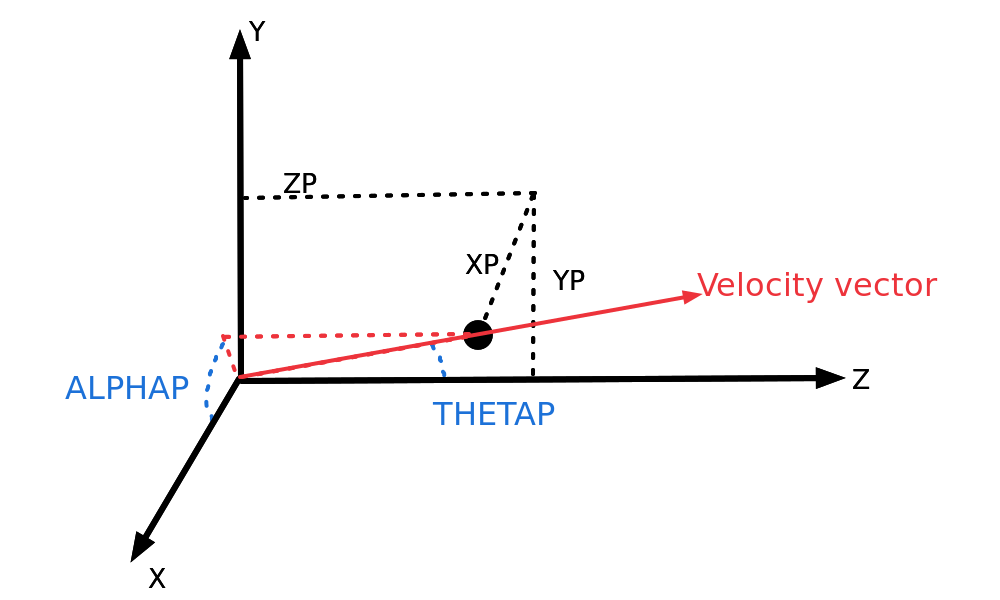
\includegraphics[width = 0.4\textwidth]{figures/coordinate_system_explanation.png}
    \caption{Illustration showing the coordinate and velocity system used in the program.}
    \label{fig:coordinate system}
\end{figure}

\clearpage

\subsubsection{Bombardment Initialization}
\label{sec:bombardment initialization}

Here, a number of initialization steps are taken to prepare for the bombardment simulation. First, the random number generator is initialized to the system time divded by three (line 198). \textbf{It is not clear why this value is divided by three}. This only happens once for every 200 simulations. \par

\begin{minted}[breaklines,fontsize=\tiny,mathescape=false,linenos,firstnumber=194]{quickbasic.py:QuickBASICLexer -x}


    FOR SIMUL = 1 TO SIMULS    ‘starting the bombardment 
    
        IF SIMUL - 200 * INT(SIMUL / 200) = 0 THEN RANDOMIZE TIMER / 3  ‘change random number seed every 200 particles
\end{minted}

Then, depending on whether the bombardment projectile is an ion or an electron (line 201 and 216), a number of particle collision data arrays are initialized with the energy, mass, and charge (lines 202-211 and lines 217-225 for electrons and ions, respectively) specified by the user, as well as the particle type. All particles are started at x,y,z = 0. \par
\begin{minted}[breaklines,fontsize=\tiny,mathescape=false,linenos,firstnumber=199]{quickbasic.py:QuickBASICLexer -x}
    

        IF iontype = 1 THEN 'iontype=1 means electron irradiation, lines 225 to 236 are for initial projectile conditions
            XP(1) = 0 ‘projectile starting location is at the original point with X=0
            YP(1) = 0 ‘projectile starting location is at the original point with Y=0
            ZP(1) = 0 'projectile starting location is at the original point with Z=0
            CP(1) = ElecCP   ‘electron charge
            mp(1) = Elecmassp 'electron mass
            THETAP(1) = 0 ‘initial incident direction is along the z axis
            ALPHAP(1) = 0 ‘initial projected direction vector is zero degree from x-axis
            EP(1) = ElecE0 ‘initial electron energy in keV
            Ptype(1) = 1  ‘particle type is electron
            correctFactor = 1  
    
        ELSE
        END IF
    
        IF iontype = 0 THEN 'iontype=0 means ion irradiation
            XP(1) = 0 ‘projectile starting location is at the original point with X=0
            YP(1) = 0 ‘projectile starting location is at the original point with Y=0
            ZP(1) = 0  ‘projectile starting location is at the original point with Z=0
            CP(1) = CP ‘projectile charge, i.e. CP=14 for silicon 
            mp(1) = massp ‘projectile mass, i.e. massp=28 for silicon
            THETAP(1) = 0  ‘initial incident direction is along the z axis
            ALPHAP(1) = 0  ‘initial projected direction vector is zero degree from x-axis
            EP(1) = INELAB 'initial ion bombardment energy in keV
            Ptype(1) = 0 ‘particle type is ion
        ELSE
        END IF
\end{minted}
\textbf{Finally, the Scan array is populated with some information. The exact purpose of this is not known.}
\begin{minted}[breaklines,fontsize=\tiny,mathescape=false,linenos,firstnumber=228]{quickbasic.py:QuickBASICLexer -x}
        'scanning ===============================
    
        FOR i = 0 TO sizeScan 'scanning
            FOR j = 0 TO sizeScan 'scanning
                '   Scan(i, j, 1) = e_deltaLat * (i - sizeScan / 2) 'scanning
                '  Scan(i, j, 2) = e_deltaLat * (i - sizeScan / 2) 'scanning
                Scan(i, j, 1) = scandelta * (i - sizeScan / 2) 'scanning
                Scan(i, j, 2) = scandelta * (j - sizeScan / 2) 'scanning
    
                Scan(i, j, 3) = 0 'depth scanning
                Scan(i, j, 4) = 0 'theta scanning
                Scan(i, j, 5) = 0 'alpha scanning
                Scan(i, j, 6) = ElecE0 'E scanning
                Scan(i, j, 7) = 0
    
            NEXT j 'scanning
        NEXT i 'scanning
        'scanning ======================
\end{minted}
\subsubsection{Bombardment bounds checking}
\label{sec:bounds checking}

At this point, several variables are assigned. The "rum" variable is particularly important, as it is used for tracking recursive bombardment. When the initial particle is simulated, it has a "rum" value of 1. But when that particle hits another particle and transfer enough energy to cause it to begin moving like a projectile, it is given a value of "rum + 1", or a "rum" value of 2. This variable is used to track how deeply the particle collisions cascade. Due to the nature of the program, the maximum cascade depth is 2000, which was mentioned earlier on. \par

The substrate atomic mass, charge, and density are also assigned to simulation variables. \textbf{The reason why the original variables are not used is not clear.} The presence of the "100" label is used by other portions of the code to jump to new projectile calculations. Something else to note is the check to see if "rum" has a value of 0. If so, this indicates, that all collision calculations are complete, and the program can move on to simulating the next collision. \par

Some bounds checking statements are then run to ensure that the particle has not done any of the follwing:

\begin{enumerate}
    \item Flown out of the window: If the Z-position of the particle is greater than the size of the plotting window (SUBWINDOW), then the particle no longer needs to be simulated. The "rum" variable is decremented, as the current cascade depth is terminated, and the simulation continues simulating the "parent" (the particle which caused the current one to cascade).
    \item Scattered off the surface: If the Z-position of the particle is less than 0, then the particle bounced off the surface of the substrate. This is considered a back-scattered particle, which no longer needs to be simulated. A counter tracking the number of backscattered particles (SPUTTER) is incremented to account for the particle, and the simulation continues to the parent particle.
\end{enumerate}

\begin{minted}[breaklines,fontsize=\tiny,mathescape=false,linenos,firstnumber=246]{quickbasic.py:QuickBASICLexer -x}
    

        rum = 1        ‘the first simulation of a new bombardment event 
        MASS2 = MASSSUB  ‘substrate atomic mass
        Z2 = ZSUB  ‘substrate atomic number (charge)
        DENSITY = SUBDENSITY ‘substrate density
    
        100
        IF rum = 0 THEN GOTO 600 ' If all collisions caused by one bombardment are finished,  start a new bombardment by jumping to 600
    
        IF ZP(rum) >= SUBWINDOW THEN 
            rum = rum – 1 ‘if electron/ion fly out of the window, stop the simulation and point to the next collision saved but not finished. 
            GOTO 100 ‘jumping to the saved collisions not yet finished. If one ion bombardment creates 900 displacements and if rum= #900 finished the collision, the pointer moves to #899 to finish the rest of collisions. #0 after rum=rum-1 means all collisions have finished. 
        ELSE
        END IF
        IF ZP(rum) < 0 THEN   ‘for the case that the particle is backscattered
            IF Ptype(rum) = 0 THEN SPUTTER = SPUTTER + 1  ‘if backscattered particle is ion, sputtering number increases by 1
            rum = rum – 1 ‘with backscattering or sputtering, no need to continue the collision, pointer moves to the next saved collision not yet finished. 
            GOTO 100
    
    
        ELSE
        END IF
\end{minted}
\subsubsection{Grouping number changes}

The code uses an optimization technique where several groups of "flying distances" (Essentailly, the random distance a projectile travels between atoms) are processed together in a group with a size of the variable "flyC". In the case of electrons, at low energies, this technique may slightly overestimate the amount of energy lost in a bombardment, resulting in a negative electron energy. This barrier is set to the value of the variable "flyjudge" multiplied by the value of the electron stopping energy (e\_stopping). To avoid this situation, the number of groupings are changed to a value (fly0) to allow for a more accurate simulation. \par

A different problem may arise for high energy electrons, where if an electron energy is beyond a certain value (EMAX), it may travel too far in a single flying distance grouping. \textbf{The exact reason why this is a problem is not known.} Because of this, the number of flying distances grouped is changed to a value to avoid this (fly0). \par

In all other cases, the number of groupings is set to fly1. \par

\textbf{There are a number of issues with this portion of the code however. Contrary to the comments, the value of fly0 and fly1 are equal (1000) and are not changed at any point in the code. Also, the value of flyjudge is also not changed, and is set to 1 at the start of the code. The result is that the value of flyC is always 1000 regardless of the energy of the projectile.}

\begin{minted}[breaklines,fontsize=\tiny,mathescape=false,linenos,firstnumber=269]{quickbasic.py:QuickBASICLexer -x}

    
        IF Ptype(rum) = 1 AND EP(rum) < flyjudge * e_stopping THEN flyC = fly0   ‘if the projectile is an electron and if the electron energy is smaller than a value, the number of flying distances to be combined for evaluation is set to be fly0.  The critical value is flyjudge X e_stopping.  Flyjudge is a number defined in the input. e_stopping is the value simulations stop when electron energy is reduced to this value.  This command is used to avoid the situation that final electron energy become negative when the flying distance combination overestimates the energy loss. 
        IF Ptype(rum) = 1 AND EP(rum) >= flyjudge * e_stopping THEN flyC = fly1 ‘if the projectile is an electron and if electron energy is above flyjudge X e_stopping, the number of flying distances to be combined is fly1. This is to allow flying distance combination if electron energy is not too low.
        IF Ptype(rum) = 1 AND EP(rum) > EMAX THEN flyC = fly0  “if the energy of the electron is above EMAX, the number of combined free flying distance is fly0. This is used to avoid the situation that flying distance combination become too long as very high energy since a single free flying distance is large at high energy. 
\end{minted}
\subsubsection{Stopped particle information}
\label{sec:stopped particle}
If a particle's energy is reduced to less than the threshold energies (e\_stopping for electrons, ion\_stopping for ions), then the particle's information is stored and written to the output data array (e\_output). \par

The radial stopping distance from the z-axis is calculated using Equation \ref{eq:radial distance} and stored as the variable "E0" and the longitudinal depth (z-position) is stored as "E1" from the arry ZP. \par

\begin{equation}
    z = \sqrt{x^2 + y^2} 
    \label{eq:radial distance}
\end{equation}

A check is performed to ensure that the electron is inside of the plotting area. Once that is confirmed, the location of the stopped electron is recorded in the "e\_output" array. This array has dimensions "e\_interval $\times$ e\_interval $\times$ 4", where e\_interval is a constant with a value of 30. The third dimension corresponds to different data type, where \textbf{"1" is the number of stopped electrons, "2" is the location where energy was lost from an electron, "3" is the location where elastic occursed, and "4" is the location of vanacies caused by electron bombardment.} This essentially divides an area of interest, defined by the "e\_range" constant (Currently set to \SI{80000000}{\angstrom}) into 30 slices along the z-axis. In each of these slices are 30 concentric rings that expand out from the z-axis. The slice that an electron stops in is determined by INT(1 + E1 / e\_deltaDep), while the ring that it stops in is found using INT(1 + E0 / e\_deltaLat). e\_deltaDep is defined as e\_range/e\_interval, or approximately \SI{2666666}{\angstrom} This is the width of each slice, and the radial separation of each ring. When, for example, an electron stops in a particular slice, the code below increments the element in the array to record the fact that an electron stopped in that slice. This information can later be used for analysis. \par

\begin{minted}[breaklines,fontsize=\tiny,mathescape=false,linenos,firstnumber=274]{quickbasic.py:QuickBASICLexer -x}

    
        ''    IF mp(rum) = MASS2 THEN PRINT #4, USING "##.###^^^^^ ##.###^^^^^ ##.###^^^^^"; XP(rum); YP(rum); ZP(rum) 'modified 01/12/01
        ''    I(INT(ZP(rum))) = I(INT(ZP(rum))) + 1
        ''   IF mp(rum) = massp THEN PR(INT(ZP(rum))) = PR(INT(ZP(rum))) + 1
        '       IF Ptype(rum) = 1 THEN PRINT #5, USING "##.###^^^^^ ##.###^^^^^ ##.###^^^^^"; XP(rum); YP(rum); ZP(rum)
        '       IF Ptype(rum) = 1 THEN ePR(1 + INT(ZP(rum) / ePRbin)) = ePR(1 + INT(ZP(rum) / ePRbin)) + 1
        IF Ptype(rum) = 1 AND EP(rum) < e_stopping THEN    ‘saving information if electrons stop. e_stopping is the threshold energy
    
            E0 = (XP(rum) ^ 2 + YP(rum) ^ 2) ^ 0.5 ‘radial distance from z axis
            E1 = ZP(rum)   ‘longitudinal depth of electrons when stopping
            IF E0 < SUBWINDOW AND E1 > 0 AND E1 < SUBWINDOW THEN ‘if electrons are in the valid region, not sputtered, and not beyond the window
                e_output(INT(1 + E0 / e_deltaLat), INT(1 + E1 / e_deltaDep), 1) = e_output(INT(1 + E0 / e_deltaLat), INT(1 + E1 / e_deltaDep), 1) + 1  ‘adding one to the saved counts at the 2-D position matrix of lateral distance and longitudinal depth. Both distances are divided by lateral direction interval (e_deltaLat) and longitudinal direction interval (e_deltaDep). Both intervals are predefined. INT() is to obtain the integral portion of a real number. 
            ELSE
            END IF
            rum = rum – 1   ‘after the stopped electron finishes the position counting, move to the previously saved not-yet-finished ion/atom, by pointing the index number to rum-1. 
            GOTO 100 ‘go back to start the next particle (other particles not-yet-finished, but produced from the same bombardment)
    
    
        ELSE
        END IF
\end{minted}
Notably, the code performs an identical action even if the projectile type is an ion. \textbf{It seems that, contrary to the comments and naming schemes of the variables, e\_output is used to store information on ions as well.}
\begin{minted}[breaklines,fontsize=\tiny,mathescape=false,linenos,firstnumber=295]{quickbasic.py:QuickBASICLexer -x}

        IF Ptype(rum) = 0 AND EP(rum) < ion_stopping THEN    ‘check if the new particle is an atom and the energy is below the threshold value
    
            E0 = (XP(rum) ^ 2 + YP(rum) ^ 2) ^ 0.5   ‘if yes, calculate the radial distance from z axis
            E1 = ZP(rum)  ‘longitudinal depth of electrons at the stopping position
            IF E0 < SUBWINDOW AND E1 > 0 AND E1 < SUBWINDOW THEN ‘judge if the ion stoops between two boundaries, surface and the maxim depth
                e_output(INT(1 + E0 / e_deltaLat), INT(1 + E1 / e_deltaDep), 4) = e_output(INT(1 + E0 / e_deltaLat), INT(1 + E1 / e_deltaDep), 4) + 1  ‘if yes, saving one count to 2-D position matrix (lateral position, longitudinal position). Both positions are divided by an distance interval. e_deltaLat is for the lateral and e_deltaDep is for the longitudinal 
            ELSE
            END IF
            rum = rum – 1  ‘after the stopped atom finishes the position counting, move to the previously saved not-yet-finished collision, by pointing the index number to rum-1. 
            GOTO 100 ‘go back to start the next particle (other particles not-yet-finished, but produced from the same bombardment)
    
    
        ELSE
        END IF
\end{minted}
\subsubsection{Electronic stopping}
\label{sec:electronic stopping}

This portion of the code calculates a collosion of an ion. First, a number of collision calculation parameters are calculated using the following equations:

\begin{equation}
    K_L = \frac{1.212\cdot Z_1^{7/6}\cdot Z_2}{(Z_1^{2/3} + Z_2^{2/3})^{3/2}m^{1/2}}
    \label{eq:first electronic stopping parameter}
\end{equation}

where $K_L$ is the first electronic stopping parameter, $Z_1$ is the atomic charge of the incident ion, $Z_2$ is the atomic charge of the substrate, and $m$ is the mass of the incident ion. \par

\begin{equation}
    S_E = K_L \sqrt{E}
\end{equation}

is the electronic stopping energy, where $E$ is the incident ion energy in eV. \par

\begin{equation}
    L = \sqrt[1/3]{\rho}
\end{equation}

$L$ is the average atomic distance in the substrate in \si{\angstrom}, and $\rho$ is the density of the substrate, in \si{atoms/\angstrom^{3}}.

\begin{equation}
    P = \sqrt{\frac{R}{\pi \cdot \rho^{2/3}}}
\end{equation}

is a collision parameter $R$ is a random number between 0,1, including 0 and excluding 1. [0,1).

\textbf{A significant potential problem is the fact that the CP variable overrides the CP array. Whether this effects the behavior of the code is not clear.}

\begin{minted}[breaklines,fontsize=\tiny,mathescape=false,linenos,firstnumber=310]{quickbasic.py:QuickBASICLexer -x}   

    
        '================== BEGIN A NEW COLLISION
    
        IF Ptype(rum) = 0 THEN ‘check if the new collision is for an atom, instead of an electron
            KL = 1.212 * CP(rum) ^ (7 / 6) * Z2 / (CP(rum) ^ (2 / 3) + Z2 ^ (2 / 3)) ^ (3 / 2) / (mp(rum) ^ .5) ‘parameter for electronic stopping
            PL = .5  ‘another parameter for electronic stopping
            SE = KL * (EP(rum) * 1000) ^ PL 'electronic stopping at energy EP(), in the unit of eV
            L = DENSITY ^ (-1 / 3) ‘average atomic distance of the target, in the unit of Angstrom
            P = (RND / (PI * DENSITY ^ (2 / 3))) ^ .5  ‘using random number RND to select a collision parameter
\end{minted}

The energy after electron energy loss is found using:

\begin{equation}
    E_P = E_{P0} - \frac{1.59\cdot L \cdot \rho \cdot S_E}{\SI{1000}{eV/keV}}
\end{equation}

where $E_{P0}$ is the pre-collision energy. 

\begin{minted}[breaklines,fontsize=\tiny,mathescape=false,linenos,firstnumber=320]{quickbasic.py:QuickBASICLexer -x}   

    
            '================== COLLISON PARAMETER
    
            EP(rum) = EP(rum) - 1.59 * L * DENSITY * SE / 1000 ‘get an updated energy after considering electron energy loss. L is the average atomic distance selected as the step length. DENSITY is the atomic density in the unit of atoms per angstrom  ^3. SE is the electronic stopping power. 1/1000 is to convert the energy loss from eV to keV
\end{minted}

Once the electronic energy loss is calculated, a check is performed to determine if the ion has stopped. If the energy of the particle is less than the "ion\_stopping" variable, then the ion is considered stopped. The "rum" counter is decremented to indicate a finished collision, and the code jumps up to the "100" label on line 239 (Section \ref{sec:bounds checking}) to continue calculations on another projectile.

\begin{minted}[breaklines,fontsize=\tiny,mathescape=false,linenos,firstnumber=325]{quickbasic.py:QuickBASICLexer -x}   

            IF EP(rum) < ion_stopping THEN ‘check again if adding electronic stopping leads to  ion stopping. Ion_stopping is the energy criteria to stop. The stopping criteria is not necessary to be threshold displacement energy
                rum = rum – 1 ‘after the stopped atom finishes the position counting, move to the previously saved not-yet-finished collision, by pointing the index number to rum-1. 
    
                GOTO 100 ‘go back to start the next particle (other particles not-yet-finished, but produced from the same bombardment)
            ELSE
            END IF
\end{minted}

At this point in the code, the recoil direction of the incident ion, as well as the direction of a knocked off atom from the substrate (if there is one), is found using the "TMAGIC" function. The results from TMAGIC are stored in three "hidden" variables, "THETA1RELATIVE", "THETA2RELATIVE", and "RE". These represent the projectile's deviation angle from the projectile velocity vector, the deviation from the projectile's velocity vector of the target atom, and the energy transferred from the projectile to the target atom, respectively. TMAGIC calculated these values using the incident ion mass, atomic charge, substrate mass, substrate charge, ion energy, and the collision parameter. \par

The results of TMAGIC are then passed to a function called "AMAGIC" to convert the relative projectile angle to values relative to the main coordinate system. This function takes the projectile's velocity vector angle relative to the z axis (THETAP) and the angle relative to the x axis on the yz plane (ALPHAP), as well as the relative angles of THETA1RELATIVE and THETA2RELATIVE. It then returns the the absolute z (THETA1) and x (ALPHA1) of the projectile, as well as the absoluate z (THETA2) and x (ALPHA2) of the target atom. Figure \ref{fig:relative angles explanation} illustrates this idea.

\begin{figure}[h]
    \centering
    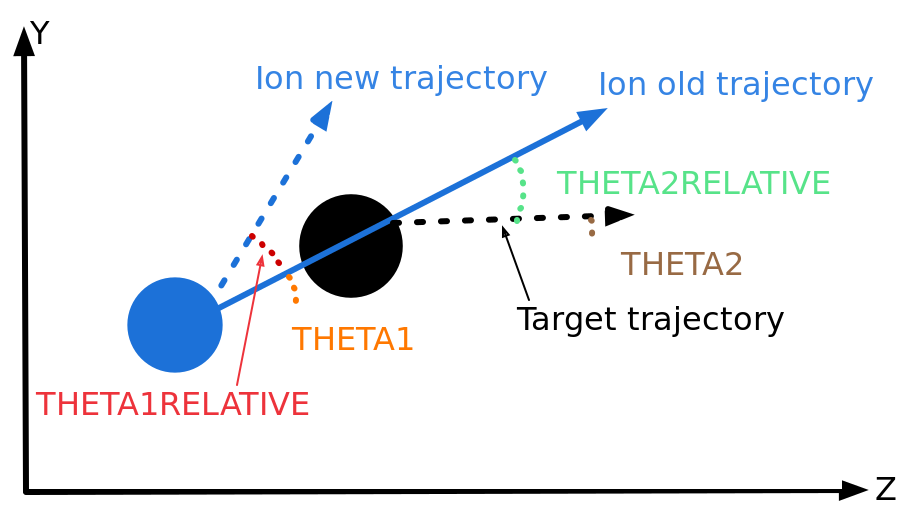
\includegraphics[width = 0.5\textwidth]{figures/relative_angles_explanation.png}
    \caption{An illustration of the relative and absolute angles discussed when explaining TMAGIC and AMAGIC. The projectile ion is illustrated in light blue, while the target atom is shown in black. This is a 2-dimensional view, only concerning the angle relative to the Z-axis (THETA).}
    \label{fig:relative angles explanation}
\end{figure}

\begin{minted}[breaklines,fontsize=\tiny,mathescape=false,linenos,firstnumber=332]{quickbasic.py:QuickBASICLexer -x}   
            CALL TMAGIC(mp(rum), CP(rum), MASS2, Z2, EP(rum), P)  
            'TO get recoil energy RE, deviation angle from the incident direction for the projectile THETA1RELATIVE, , recoil direction of target atom with respect to the incident direction THETA2RELATIVE
            CALL AMAGIC(THETAP(rum), ALPHAP(rum), THETA1RELATIVE, THETA2RELATIVE)  ‘obtain the new directions with respect to the original xyz coordinate for the projectile and target atom (THETAP is the angle away from the z axis, ALPHAP is the angle away from the x axis on YZ plane); THETAP(RUM), ALPHA(RUM) are angles before collision; THETA1 and THETA2 are new angles relative to the direction before the collision
\end{minted}

This portion of the code saves information regarding the collision to the target atom (rum + 1). The position of the target is stored as the position of the incident ion, offset by the atomic separation in the direction of the ion's velocity vector. The target charge is then set to the value for the substrate. The target mass is set to the mass of the substrate. This is logical, as the target atom will naturally be one of the substrate atoms. The target velocity angle (THETA2, ALPHA2), as well as the energy (RE) are assigned to the target.

\begin{minted}[breaklines,fontsize=\tiny,mathescape=false,linenos,firstnumber=335]{quickbasic.py:QuickBASICLexer -x}   
            
            '=====TEMPERARY SAVE INFORMATION.  Using matrix at index rum+1 to save everything about the target. Note the information about project is save with index rum
    
            ZP(rum + 1) = ZP(rum) + L * COS(THETAP(rum))   ‘assign new depth to target
            XP(rum + 1) = XP(rum) + L * SIN(THETAP(rum)) * COS(ALPHAP(rum)) ‘assign new X to target 
            YP(rum + 1) = YP(rum) + L * SIN(THETAP(rum)) * SIN(ALPHAP(rum)) ‘assign new Y to target
            CP(rum + 1) = Z2 'CP(rum + 1) = CP(rum)   ‘transfer target charge information
            mp(rum + 1) = MASS2 'mp(RUM + 1) = mp(RUM)  ‘transfer target mass information
            THETAP(rum + 1) = THETA2   ‘transfer angle information of Recoiled target. Note “2” for target. THETA2 is a shared parameter obtained from subroutine AMAGIC 
            ALPHAP(rum + 1) = ALPHA2 'transfer angle information of  Recoiled target. Note “2” for target. ALPHA2 is a shared parameter obtained from subroutine AAMAGIC
            EP(rum + 1) = RE  ‘transfer recoil energy to target atom energy. RE is a shared parameter obtained from subroutine TMAGIC
\end{minted}

\subsubsection{Plotting}
\label{sec:ion plotting}

A few lines of code for plotting are shown here. First, a window is drawn, and then some text displaying the number of simulations run so far. \par

Following that, a line is drawn in the window (which is a 630 $\times$ 330 pixel window) from $x_1 = \text{round}\left(\frac{z}{x_{\text{total}\cdot w_x}}\right)$ and $y_1 = \text{round}\left(0.5 + \frac{x}{y_{\text{total}}\cdot w_y}\right)$ to $x_2 = \text{round}\left(\frac{z_t}{x_{\text{total}\cdot w_x}}\right)$ and $y_2 = \text{round}\left(0.5 + \frac{x_t}{y_{\text{total}}\cdot w_y}\right)$, where $z$ is the z-position of the incident ion (ZP(rum)) in \si{\angstrom}, $x$ is the x-position of the incident ion (XP(rum)) in \si{\angstrom}, $x_{\text{total}}$ is the total length of the plotting window in \si{\angstrom} (SUBWINDOW), $y_{\text{total}}$ is the total height of the plotting window in \si{\angstrom} (SUBWINDOW), $w_x$ is the number of pixels in the x-direction for the plotting window (WINDOWX), and $w_y$ is the number of pixels in the y-direction for the plotting window (WINDOWY). \par

If the mass of the particle is equal to that of the incident ion, the line is drawn in red. In the case that the mass of the projectile is equal to that of the substrate, the line is drawn white (color code "1"). \textbf{Note that for self-bombardment, where the ion and the substrate are the same atom, both lines will be drawn. Since the "white line" command comes later, it will likely draw over the red line.}

\begin{minted}[breaklines,fontsize=\tiny,mathescape=false,linenos,firstnumber=346]{quickbasic.py:QuickBASICLexer -x}   

    
            WINDOW SCREEN(0, 0)-(WINDOWX, WINDOWY)  ‘define/draw a window
    
            LOCATE 4, 47 ‘locate position for words below
            PRINT " SIMULATION:"; SIMUL; "("; SIMULS; ")" 'provide updates on how many finished out of the total

    
            IF mp(rum) = massp THEN LINE (INT(ZP(rum) / SUBWINDOW * WINDOWX), INT((0.5 + XP(rum) / SUBWINDOW) * WINDOWY))-(INT(ZP(rum + 1) / SUBWINDOW * WINDOWX), INT((0.5 + XP(rum + 1) / SUBWINDOW) * WINDOWY)), 4 'draw a short line from previous position to the current position. Note all positions are normalized by the window size and then change to correct pixel number. The drawing is for projectile ion
            IF mp(rum) = MASSSUB THEN LINE (INT(ZP(rum) / SUBWINDOW * WINDOWX), INT((0.5 + XP(rum) / SUBWINDOW) * WINDOWY))-(INT(ZP(rum + 1) / SUBWINDOW * WINDOWX), INT((0.5 + XP(rum + 1) / SUBWINDOW) * WINDOWY)), 1 'similar to the above but the drawing is for target atoms with a different color
\end{minted}

\subsubsection{Projectile update}

In the case that the transferred energy (RE) is not enought to displace the target atom, the code updates the original projectile with new position and velocity information. The particle assumes the position of the target, and is given the updated velocity vecotr direction from the AMAGIC function (THETA1, ALPHA1). The new energy of the projectile is assigned by subtracting RE from the energy of the projectile. \par

The simulation will continue calculating the collision information for current particle, and will jump back to the "100" label on line 239 (Section \ref{sec:bounds checking}). 

\begin{minted}[breaklines,fontsize=\tiny,mathescape=false,linenos,firstnumber=356]{quickbasic.py:QuickBASICLexer -x}   

    
    
            IF RE <= ion_Ed THEN ‘if target atom energy is too low. No need to save information for target since there is no displacement. Saved information in rum+1 for the target is “selectively” transferred back to rum for the projectile.  
                ZP(rum) = ZP(rum + 1)  ‘return new Z back to projectile as an update
                XP(rum) = XP(rum + 1) ‘return new X back to projectile as an update
                YP(rum) = YP(rum + 1)  ‘return new Y back to projectile as an update
                mp(rum) = mp(rum)  ‘keep the original projectile mass
                CP(rum) = CP(rum) ‘keep the original projectile charge
                THETAP(rum) = THETA1  ‘update on the new direction for projectile, obtained from AMAGIC
                ALPHAP(rum) = ALPHA1 ‘update on the new direction for projectile, obtained from AMAGIC
                EP(rum) = EP(rum) - RE ‘update energy for projectile, considering energy transfer to the target. RE obtained from TMAIG
                GOTO 100    ‘return for the next step with new position and new energy. Note the index is kept at rum. It means the pointer stays on the same projectile.  All previous saved information on rum+1 are not used if target atom does not become a displacement
            ELSE
            END IF
\end{minted}

\subsubsection{Target cascade calculations}

In the case that RE was large enough to cause a displacement, the same assignments as before are made for the current particle. \textbf{This is not necessary, since the same assignments are done whether a cascade happens or not.}

\begin{minted}[breaklines,fontsize=\tiny,mathescape=false,linenos,firstnumber=371]{quickbasic.py:QuickBASICLexer -x}   

            '====IF RE>0.02  A target displacement is created. The new atom needs to be assigned with rum+1.  From lines 411 to 420, the information transfer for rum+1 already happened. So, only the projectile needs to be updated for rum
    
            XP(rum) = XP(rum + 1)    ‘projectile has the same X as the target
            YP(rum) = YP(rum + 1) 'YP(RUM) = YP(RUM + 1) ‘projectile has the same Y as the target
            ZP(rum) = ZP(rum + 1) 'ZP(RUM) = ZP(RUM + 1) ‘projectile has the same Z as the target
            mp(rum) = mp(rum) 'projectile keeps its original mass
            CP(rum) = CP(rum) 'projectile keeps its original charge
            THETAP(rum) = THETA1 'projectile has its updated angle, obtained from AMAGIC. “1” is for projectile. TEHTA1 is shared from AMAGIC
            ALPHAP(rum) = ALPHA1 'projectile has its updated angle, obtained from AMAGIC. “1” is for projectile. ALPHA1 is shared from AMAGIC
            EP(rum) = EP(rum) - RE 'new energy considering the recoil energy loss
\end{minted}

Here, since the target atom is displaced, the vanacy created must be accounted for. In order to do this, the code checks whether the displaced particle is inside the range of interest. If so, a process very similar to that found in Section \ref{sec:stopped particle} is used to set the e\_output vacancy data. \par

Following that, rum is then incremented to focus the simulation calculations on the target particle that was displaced. The program then jumps to the "100" label on line 239 (Section \ref{sec:bounds checking}) to continue calculations for the cascaded particle.

\begin{minted}[breaklines,fontsize=\tiny,mathescape=false,linenos,firstnumber=382]{quickbasic.py:QuickBASICLexer -x}   

            IF ZP(rum + 1) > 0 AND ZP(rum + 1) < SUBWINDOW THEN  ‘Since one displacement occurs, vacancy information needs to be saved, if the displacement position is within two boundaries: surface and backside.
                '            V(INT(ZP(rum + 1))) = V(INT(ZP(rum + 1))) + 1  ‘optional for vacancy counting 
                E0 = (XP(rum) ^ 2 + YP(rum) ^ 2) ^ 0.5   ‘distance away from z axis
                E1 = ZP(rum)  ‘depth along z axis
                e_output(INT(1 + E0 / e_deltaLat), INT(1 + E1 / e_deltaDep), 4) = e_output(INT(1 + E0 / e_deltaLat), INT(1 + E1 / e_deltaDep), 4) + 1  ‘adding one vacancy into output matrix for e_output (Lateral, Longitudinal, 4). “4” is for vacancy. e_deltaLat and e_deltaDep are distance interval. INT is for taking integral number. 
    
            ELSE
            END IF
            rum = rum + 1   ‘since a new energetic atom is produced and taking the index rum+1, the calculation pointer is re-appointed to rum+1
            GOTO 100   ‘restart a new calculation with pointer at rum+1. If a displacement is created. The newly displaced atom will finish the simulation. Then the pointer moves back to the projectile to continue
        ELSE
        END IF
\end{minted}

\subsection{Electron irradiation}

All of the code in Section \ref{sec:ion bombardment} was for ion bombardment. This portion of the code focuses on electron bombardment. This is a significantly more complicated task, as several different computationally intensive tasks must be performed in order to calculate electron bombardment. In particular, Mott scattering must be calculated, which takes a great deal of computation time. A number of optimiziations are made to reduce the computational cost of these calculatiosn, most notably the "flying distance grouping method". This method assumes that Mott scattering results in such a small energy loss that it can be assumed to be negligible for groups of flying distances, provided that the total flying distance is sufficiently small. Using this assumption, the same energy can be used for all of the calculations for a group of flying distances. This greatly reduces computation time, as the Mott scattering total cross-section does not have to be recalculated for every flying distance, which is computationally expensive. \par 

\subsubsection{Flying distace creation}

A single group of flying distances is generated using random numbers. An array "RL" with a size corresponding to the variable "flyC" is used to store random numbers to be used to calculate the flying distances.

\begin{minted}[breaklines,fontsize=\tiny,mathescape=false,linenos,firstnumber=395]{quickbasic.py:QuickBASICLexer -x}
    
        'Below is for electron irradiation
    
        IF Ptype(rum) = 1 THEN   ‘”1” means the particle is electron
    
            FOR trial2 = 1 TO flyC   ‘create a chain of random number for free flying distance within the group.  flyC is the number of free flying distances in the group
                '    RANDOMIZE TIMER / 3   
                RL(trial2) = RND    ‘Assigned random number to random number matrix with ID of trial2. Trial2 starts from 1, increase till flyC. 
            NEXT trial2     ‘repeat until all numbers are assigned
\end{minted}

The randomly generated numbers are then sorted in acending order. The following is an implementation of the bubble sort algorithm. More on the bubble sort algorithm: \href{https://en.wikipedia.org/wiki/Bubble_sort}{Bubble Sort Wikipedia Page}

\begin{minted}[breaklines,fontsize=\tiny,mathescape=false,linenos,firstnumber=404]{quickbasic.py:QuickBASICLexer -x}

            FOR trial3 = 1 TO flyC – 1   ‘first step to rank random number from low to high. Here is to pick from the original order.
                FOR trial4 = trial3 + 1 TO flyC  ‘compare with the rest after the one being picked 
                    IF RL(trial3) > RL(trial4) THEN  ‘judge whether there is random number behind is smaller than the picked one
                        temp = RL(trial3)  ‘assign a tempera saving for the originally picked number
                        RL(trial3) = RL(trial4)  ‘assigned the smaller random number to the originally picked one
                        RL(trial4) = temp  ‘transfer the save value of the original random to the one being swapped
                    END IF
                NEXT trial4   ‘finish everyone behind trial3
            NEXT trial3  ‘finish all trial3 from 1 to fly-1
\end{minted}

\subsubsection{Mott scattering integrated cross section calculation}

The total Mott scattering cross section is calculated here. The maximum scattering angle is \SI{180}{\degree}, so this range is divided into 1000 intervals. Because the Mott scattering cross section increases rapidly at small angles, a non-uniform distribution was used for calculating small-angle scattering with higher resolution than large angle scattering. \par

The DSCMOTT subroutine is used to calculate the Mott Scattering differential cross section. This is stored in the "hidden" variable called "DiffCross", which is the differential Mott scattering cross section. The function accepts the Mott scattering parameters, eletron screening parameters, electron energy, substrate atomic charge, and the angle. \par

Angles are distributed using this expression:

\begin{equation}
    \theta_i = \pi\frac{1 - 10^{i/m}}{1 - 10}
    \label{eq:angle distribution}
\end{equation}

where $i$ is the interval being calculated (ANGLE1), and $m$ is the total number of intervals (Divisor). The reason behind this uneven angle distribution is illustrated in Figure \ref{fig:shao angle distribution}. \par

\begin{figure}
    \centering
    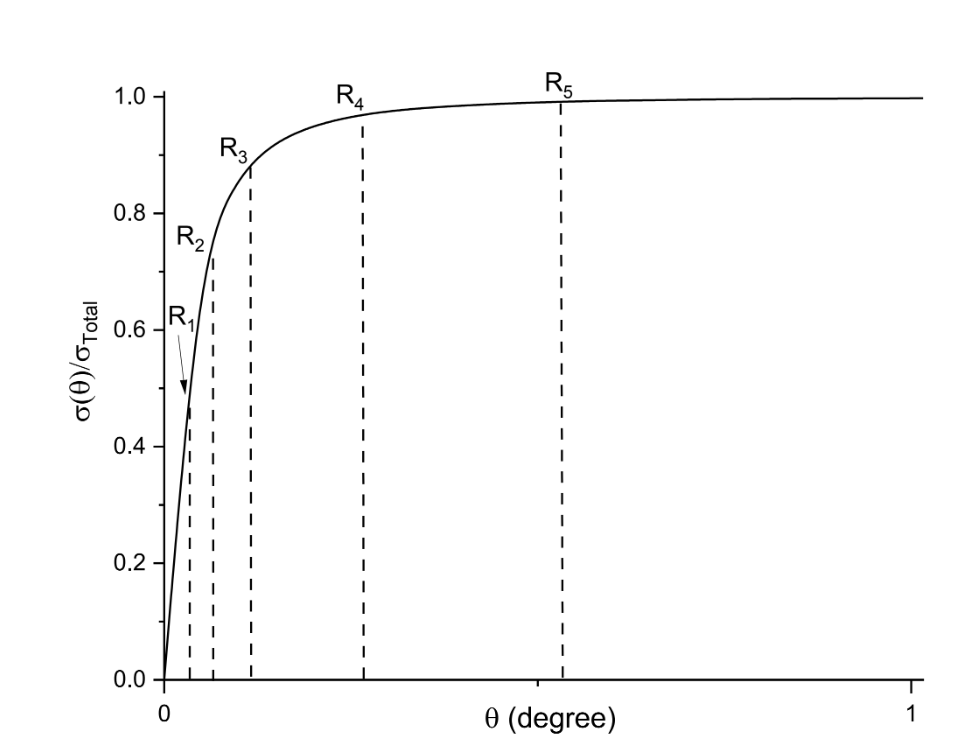
\includegraphics[width = 0.5\textwidth]{figures/shao angle distribution.png}
    \caption{Obtaining $\theta_i$ values for each $R_i$ for a group of five random numbers in ordered sequence from low to high. (Taken from Shao.)}
    \label{fig:shao angle distribution}
\end{figure}

Depending on which angle is being calculated, different equations are used to calculate the contribution to the total cross section. For the smallest (and first angle):

\begin{equation}
    \sigma_{t} = \sigma_{t,i} + \frac{d\sigma}{d\theta}\cdot 2\pi \sin(\theta_i)\frac{\theta_2 + \theta_1}{2}
\end{equation}

and for the last (and largest) angle,

\begin{equation}
    \sigma_{t} = \sigma_{t,i} + \frac{d\sigma}{d\theta}\cdot 2\pi \sin(\theta_i)\left( \pi - \frac{\theta_{m-2} + \theta_{m-1}}{2}\right)
\end{equation}

and for all other angles,

\begin{equation}
    \sigma_{t} = \sigma_{t,i} + \frac{d\sigma}{d\theta}\cdot 2\pi \sin(\theta_i)\frac{\theta_{i+1} - \theta_{i-1}}{2}
\end{equation}

where $\sigma_{t}$ is the total Mott scattering cross section, and $\frac{d\sigma}{d\theta}$ is the differential cross section. Note that the electron energy is multiplied by a variable called "correctFactor". This variable is important, as it is used to correct the electron energy to a more accurate value than the value before scattering begins. This is part of the "mid-point approximation method" used to increase the accuracy of scattering calculations. This method will be discussed in greater detail later on.

\begin{minted}[breaklines,fontsize=\tiny,mathescape=false,linenos,firstnumber=414]{quickbasic.py:QuickBASICLexer -x}

            
            TotalCross = 0      ‘preparing to calculate integrated cross section 
            FOR ANGLE1 = 1 TO (Divisor - 1) ‘dividing 180 degrees by Divisor, performing integration
                CALL DSCMOTT(mott(), scr(), EP(rum) * correctFactor, ZSUB, PI / (1 - 10) * (1 - 10 ^ (ANGLE1 / Divisor)))    ‘obtaining differential cross section at specific angle. The angle reading is not uniform. It has higher density close to 0.
                IF ANGLE1 = 1 THEN TotalCross = TotalCross + DiffCross * 2 * PI * SIN(PI / (1 - 10) * (1 - 10 ^ (1 / Divisor))) * ((PI / 2 / (1 - 10) * (1 - 10 ^ (2 / Divisor))) + (PI / 2 / (1 - 10) * (1 - 10 ^ (1 / Divisor))))  ‘integration concerning the first interval which starts from angle=0
                IF ANGLE1 > 1 AND ANGLE1 < (Divisor - 1) THEN TotalCross = TotalCross + DiffCross * 2 * PI * SIN(PI / (1 - 10) * (1 - 10 ^ (ANGLE1 / Divisor))) * ((PI / 2 / (1 - 10) * (1 - 10 ^ ((ANGLE1 + 1) / Divisor))) - (PI / 2 / (1 - 10) * (1 - 10 ^ ((ANGLE1 - 1) / Divisor))))  ‘integration for angle intervals excluding two boundary points
                IF ANGLE1 = (Divisor - 1) THEN TotalCross = TotalCross + DiffCross * 2 * PI * SIN(PI / (1 - 10) * (1 - 10 ^ ((Divisor - 1) / Divisor))) * (PI - (PI / 2 / (1 - 10) * (1 - 10 ^ ((Divisor - 1) / Divisor))) - (PI / 2 / (1 - 10) * (1 - 10 ^ ((Divisor - 2) / Divisor))))  ‘integration concerning the last angle point concerning the boundary at 180 degree
                '    P1 = DiffCross
                '   P2 = TotalCross
                '  PRINT #11, USING "##.###^^^^^ ##.###^^^^^ ##.###^^^^^"; 180 / PI * PI / (1 - 10) * (1 - 10 ^ (ANGLE1 / Divisor)); P1; P2 'optional for saving differential cross section and integrated cross section as a function of angle, for checking 
            NEXT ANGLE1  ‘finish from 0 to 180
\end{minted}

The flying distances for the current group of electrons is calculated here. For "flyC" distances, (which has value of 1000), the flying distance is calculated using the following:

\begin{equation}
    L = -\frac{\ln(R)}{N\cdot \sigma_T}
    \label{eq:flying distance}
\end{equation}

where $L$ is the flying distance in \si{\angstrom}, $R$ is a random number between 0 (inclusive) and 1 (exclusive), [0,1), $N$ is the atomic density of the substrate in \si{atoms/\angstrom^3}, and $\sigma_T$ is the total Mott scattering cross section. The values for these flying distances are stored in the "RN" array. There is a check that assings the random number to a variable called "ForLSelect", which checks if the random number is 0. It is important that the number is not zero, as this would result in an error, as the natural logarithm in Equation \ref{eq:flying distance} of 0 is undefined. In addition, the total flying distance of the entire group is calculated by calculating the sum of all the individual flying distances and storing them in a variable called "Lselected".

\begin{minted}[breaklines,fontsize=\tiny,mathescape=false,linenos,firstnumber=426]{quickbasic.py:QuickBASICLexer -x}
    
    
    
            Lselected = 0    ‘prepare for flying distance assignment
            FOR trial1 = 1 TO flyC ‘starting flying distance assignment with the group. flyC is the group size
    
                ForLselect = RND    ‘assign random number to ForLselect
                IF ForLselect = 0 THEN ForLselect = 1E-10  ‘if random number is zero, change to a very small number
                RN(trial1) = -LOG(ForLselect) / (SUBDENSITY * 1E24 * TotalCross) + (SUBDENSITY * 1E24) ^ (-1 / 3)
                '   Random number is converted to free flying distance using total cross section obtained from integration (lines 521 to 541)
                Lselected = Lselected + RN(trial1)  ‘adding each free flying distance to get the total length of the whole group
            NEXT trial1  ‘repeat and go through all free flying distance in the group
\end{minted}

At this point, the scattering angle is calculated by performing a second integration. The program begins calculating a partial scattering cross section from the smallest to the largest angle (line 424), with the angle interavls being calculated using Equation \ref{eq:angle distribution}. It calculates a Mott partial cross section (lines 428-430), depending on the angle being considered (first, middle, or last for lines 428, 429, and 430, respectively). The total scattering angle is tracked using the "ForThetaSelect1". The previously calculated partial cross section is also stored in a variable called "ForThetaSelect0". These variables are used to re-calculate differential cross sections by taking the difference between them. \par

\vspace{0.5 cm}

Line 433 checks to see if the calculated partial cross section matches the randomly selected (and sorted) numbers found in lines 374 - 392. These random numbers represent possible Mott scattering cross sections. If the randomly selected cross section is too small, then the program advances to the next largest random number and checks it instead (lines 439, 439, and 432). Once the random number matches the calculated partial Mott scattering cross section is found, three different cases considered, and a different equation is used in each case to find the scattering angle. Note that $\Delta \theta_{i}$ is defined as follows, depending on the boundary conditions: \par

\begin{equation}
    \Delta \theta_i = \begin{cases}
        \frac{\theta_{1} + \theta_{2}}{2} &i = 0 \\
        \frac{\theta_{i + 1} - \theta_{i - 1}}{2} &0 < i < m - 1 \\
        \pi - \frac{\theta_{m - 1} - \theta_{m - 2}}{2} &i = m - 1 \\
    \end{cases}
\end{equation}

Also, in the code, $i$ is now represented by the variable "ANGLE2".\par

\vspace{0.5 cm}

In the case that the angle begin calculated is not at a boundary $2 \le i \le m - 1$ (Line 434): \par

\begin{equation}
        \theta = \frac{\theta_{i} + \theta_{i + 1}}{2} - \left[ \overbrace{\boxed{\frac{\sum_0^{\theta_{i}}\frac{d\sigma_{\text{Mott}}(\theta_{i})}{d\Omega}\cdot 2\pi\cdot \sin\theta_{i}\cdot \Delta \theta_{i}}{\sigma_T}}}^{\text{ForThetaSelect1, line 429}} - \overbrace{\boxed{R}}^{\text{RL(trial5)}} \right]\cdot \frac{\Delta \theta_{i}}{\underbrace{\boxed{\frac{d\sigma_{\text{Mott}}}{d\Omega} \cdot 2\pi \cdot\sin\theta_{i}\cdot \Delta \theta_{i}\frac{1}{\sigma_T}}}_{\text{ForThetaSelect1 - ForThetaSelect0}}}
\end{equation}

\textbf{Note that in literature provided by Dr. Shao, the angle interval is incremented by 1 in all terms (i.e. $\bm{\theta_i \rightarrow \theta_{i + 1}}$). This equation reflects what the code is doing.} \par

\vspace{0.5 cm}

In addition, note how $\frac{d\sigma_{\text{Mott}}}{d\Omega} \cdot 2\pi \cdot\sin\theta_{i}\cdot \Delta \theta_{i}\frac{1}{\sigma_T}$ is calculated. It is found by taken the difference between two adjacent calculated partial cross-sections (ForThetaSelect1 - ForThetaSelect0 = $\Delta$ ForThetaSelect): \par

\begin{equation}
    \frac{d\sigma_{\text{Mott}}}{d\Omega} \cdot 2\pi \cdot\sin\theta_{i}\cdot \Delta \theta_{i}\frac{1}{\sigma_T}  = \frac{\sum_0^{\theta_{i}}\frac{d\sigma_{\text{Mott}}(\theta_{i})}{d\Omega}\cdot 2\pi\cdot \sin\theta_{i}\cdot \Delta \theta_{i}}{\sigma_T} - \frac{\sum_0^{\theta_{i-1}}\frac{d\sigma_{\text{Mott}}(\theta_{i-1})}{d\Omega}\cdot 2\pi\cdot \sin\theta_{i-1}\cdot \Delta \theta_{i-1}}{\sigma_T}
\end{equation}

If the angle is at the left-hand boundary ($i = 1$) (Line 435):

\begin{equation}
    \theta = \frac{\theta_2 + \theta_1}{2} - \left[ \overbrace{\boxed{\frac{\frac{d\sigma_{\text{Mott}}(\theta_1)}{d\Omega}\cdot 2\pi\cdot \sin\theta_1\cdot \Delta \theta_ 1}{\sigma_T}}}^{\text{ForThetaSelect1, line 428}} - \overbrace{\boxed{R}}^{\text{RL(trail5)}}\right]\cdot \frac{\Delta\theta_1}{\underbrace{\boxed{\frac{d\sigma_{\text{Mott}}(\theta_1)}{d\Omega}\cdot 2\pi\cdot \sin\theta_{1}\cdot \Delta \theta_1\cdot \frac{1}{\sigma_T}}}_{\text{ForThetaSelect1 - ForThetaSelect0}}}
\end{equation}

Finally, if the angle is at the right-hand boundary where $i = m - 1$ (line 436):

\begin{equation}
    \theta = \pi - \left[ \overbrace{\boxed{\frac{\sum_0^{\theta_{m-1}}\frac{d\theta_{\text{Mott}}(\theta_{m -1})}{d\Omega}\cdot 2\pi\cdot \sin\theta_{m - 1}\cdot \Delta \theta_{m-1}}{\sigma_T}}}^{\text{ForThetaSelect1, line 430}} - \overbrace{\boxed{R}}^{\text{RL(trial5)}} \right] \cdot \frac{\Delta \theta_{m-1}}{\underbrace{\boxed{\frac{d\sigma_{\text{Mott}}(\theta_{m-1})}{d\Omega}\cdot 2\pi \cdot \sin\theta_{m - 1}\cdot \Delta \theta_{m-1}\cdot \frac{1}{\sigma_T}}}_{\text{ForThetaSelect1 - ForThetaSelect0}}}
\end{equation}

To terminate this process, a large value is chosen for the last random number (line 423). \textbf{Note that the code comments call this value an "angle", however it instead represents a partial Mott scattering cross section}. This is important, as if the last random number is smaller than the partial Mott scattering cross section, lines 432 and 439 would result in an infinite loop, hanging the program. Finally, ForThetaSelect0 is set to ForThetaSelect1 (line 443) to store the previous calculated Mott scattering angle. 

\begin{minted}[breaklines,fontsize=\tiny,mathescape=false,linenos,firstnumber=438]{quickbasic.py:QuickBASICLexer -x}

    
            ForThetaSelect0 = 0  ‘prepare to identify scattering angle. ThetaSelect0 is the integrated cross section. It is zero before the integration starts 
    
            trial5 = 1     ‘pointer needs to be updated
    
            RL(flyC + 1) = 12345.   ‘assignment of a “ridiculous angle” to the last scattering angle in the group
            FOR ANGLE2 = 1 TO (Divisor - 1)   ‘go through each angle point from 0 to 180
    
                CALL DSCMOTT(mott(), scr(), EP(rum) * correctFactor, ZSUB, PI / (1 - 10) * (1 - 10 ^ (ANGLE2 / Divisor)))  ‘obtain Mott differential cross section as a specific angle
    
                IF ANGLE2 = 1 THEN ForThetaSelect1 = ForThetaSelect0 + DiffCross / TotalCross * 2 * PI * SIN(PI / (1 - 10) * (1 - 10 ^ (1 / Divisor))) * ((PI / 2 / (1 - 10) * (1 - 10 ^ (2 / Divisor))) + (PI / 2 / (1 - 10) * (1 - 10 ^ (1 / Divisor))))    ‘Integration concerning first point at angle=0 needs to be specially treated. 
                IF ANGLE2 > 1 AND ANGLE2 < (Divisor - 1) THEN ForThetaSelect1 = ForThetaSelect0 + DiffCross / TotalCross * 2 * PI * SIN(PI / (1 - 10) * (1 - 10 ^ (ANGLE2 / Divisor))) * ((PI / 2 / (1 - 10) * (1 - 10 ^ ((ANGLE2 + 1) / Divisor))) - (PI / 2 / (1 - 10) * (1 - 10 ^ ((ANGLE2 - 1) / Divisor)))) ‘integration for the middle points without two angle boundaries
                IF ANGLE2 = (Divisor - 1) THEN ForThetaSelect1 = ForThetaSelect0 + DiffCross / TotalCross * 2 * PI * SIN(PI / (1 - 10) * (1 - 10 ^ ((Divisor - 1) / Divisor))) * (PI - (PI / 2 / (1 - 10) * (1 - 10 ^ ((Divisor - 1) / Divisor))) - (PI / 2 / (1 - 10) * (1 - 10 ^ ((Divisor - 2) / Divisor))))  ‘integration concerning the last boundary needs to be specially treated
    
                150
                IF ForThetaSelect1 > RL(trial5) THEN  ‘if the integration cross section is larger than the first random number, do the following
                    IF ANGLE2 > 1 AND ANGLE2 < Divisor - 1 THEN RA(trial5) = PI / 2 / (1 - 10) * (1 - 10 ^ ((ANGLE2 + 1) / Divisor)) + PI / 2 / (1 - 10) * (1 - 10 ^ (ANGLE2 / Divisor)) - (ForThetaSelect1 - RL(trial5 )) * (PI / 2 / (1 - 10) * (1 - 10 ^ ((ANGLE2 + 1) / Divisor)) - PI / 2 / (1 - 10) * (1 - 10 ^ ((ANGLE2 - 1) / Divisor))) / (ForThetaSelect1 - ForThetaSelect0)   ‘if it happens for the middle point,  corresponding angle is read from the proportionality, judged by the distance from the right side boundary point.  RA is the scattering angle selected.
                    IF ANGLE2 = 1 THEN RA(trial5) = PI / 2 / (1 - 10) * (1 - 10 ^ (2 / Divisor)) + PI / 2 / (1 - 10) * (1 - 10 ^ (1 / Divisor)) - (ForThetaSelect1 - RL(trial5)) * (PI / 2 / (1 - 10) * (1 - 10 ^ (2 / Divisor)) + PI / 2 / (1 - 10) * (1 - 10 ^ (1 / Divisor))) / (ForThetaSelect1 - ForThetaSelect0)  ‘if it happens to the first angle interval, special treatment needs since interval width differs from middle points. RA is the scattering angle selected
                    IF ANGLE2 = Divisor - 1 THEN RA(trial5) = PI - (ForThetaSelect1 - RL(trial5)) * (PI - PI / 2 / (1 - 10) * (1 - 10 ^ ((Divisor - 1) / Divisor)) - PI / 2 / (1 - 10) * (1 - 10 ^ ((Divisor - 2) / Divisor))) / (ForThetaSelect1 - ForThetaSelect0) ‘if it happens to the last angle interval, special treatment needs since the interval width differs from middle points. RA is the scattering angle selected.
                    trial5 = trial5 + 1    ‘moves to the next random point. The pointer is increased by 1 
    
                    GOTO 150     ‘go back and repeat. The last pointer value (trial5) becomes flyC+1. Random number assigned for flyC+1 in the matrix RL(flyC+1) is ‘ridiculously large’ number, to make sure “GOTO 150 will not happen after flyC+1. 
                ELSE
                END IF
    
                ForThetaSelect0 = ForThetaSelect1   ‘for integration. The integrated value is saved as the base line, to be added with the increased value from the next angle interval, to be calculated in the next angle point. 
    
            NEXT ANGLE2
\end{minted}

This portion of the code randomly arranges the scattering angles found previously. This is needed to ensure that the scattering angle doesn't strictly increase for each flying distance. The code steps back from the last element in the scattering angles array "RA", and swaps it with a random element in RA. It does this for every element, randomly shuffling the array. This is an implementation of the Fisher-Yates shuffle, or the Knuth shuffle. More on this algorithm: \href{https://en.wikipedia.org/wiki/Fisher%E2%80%93Yates_shuffle}{Fisher--Yates Shuffle}

\begin{minted}[breaklines,fontsize=\tiny,mathescape=false,linenos,firstnumber=467]{quickbasic.py:QuickBASICLexer -x}
    
    ‘lines 615 to 622 is to go through the flying distance group, from the last one to the first one, randomly pick one before the current one and switch the value. This is used to disorder the ordered scattering angle and randomly assign it them to different free flying distances. 
            FOR trial99 = flyC TO 2 STEP -1   ‘go through all distances from the last one to the first one
                jj = INT(RND * trial99) + 1    ‘randomly pick a number smaller than trial99
                qqq = RA(trial99)  ‘save scattering angle of trial99 temporarily 
                RA(trial99) = RA(jj)   ‘transfer randomly picked scattering angle to trial99
                RA(jj) = qqq  ‘transfer temporarily save value to the randomly picked free flying distance. Hence swapping finishes
            NEXT trial99  ‘go through all random number in the group
\end{minted}

\subsubsection{Energy loss calculations}

The energy transfer from Mott scattering is calculated using the following equation:

\begin{equation}
    E_t = \frac{[(E_k + m_ec^2) \sin^2\theta + Mc^2 (1 - \cos\theta)]E_k(E_k + 2m_ec^2)}{(E_k + Mc^2)^2 - E_k(E_k + 2m_ec^2)\cos^2\theta}
\end{equation}

where $E_t$ is the recoil energy in J (totalRE, in keV), $E_k$ is the electon energy in J (EP(rum) in keV), $m_e$ is the mass of an electron in kg, $c$ is the speed of light in \si{m/s}, and $M$ is the substrate mass (MASSSUB, in amu). In the code, the constants are simplified into numerical values, and converted to units so that the value of totalRE is in keV. The final energy loss is stored at index "rum" in the "RE" array. This is used later to determine if subtrate atoms are displaced. \par

\begin{minted}[breaklines,fontsize=\tiny,mathescape=false,linenos,firstnumber=475]{quickbasic.py:QuickBASICLexer -x}
    
    
            totalRE = 0   ‘prepare for the energy loss calculation 
    
            FOR trial6 = 1 TO flyC  ‘go through each free flying distance in the group
    
                ElecREup = ((EP(rum) + 511) * (SIN(RA(trial6))) ^ 2 + MASSSUB * 931 * 1000 * (1 - COS(RA(trial6)))) * EP(rum) * (EP(rum) + 2 * 511)   ‘for calculation of energy transfer 
                ElecREdown = (EP(rum) + MASSSUB * 931.5 * 1000) ^ 2 - EP(rum) * (EP(rum) + 2 * 511) * (COS(RA(trial6))) ^ 2 ‘for calculation of energy transfer
                RE(trial6) = ElecREup / ElecREdown ‘for calculation of energy transfer
                totalRE = totalRE + RE(trial6)  ‘adding all energy loss with the group
            NEXT trial6  ‘go through the whole free flying distance group 
\end{minted}

The total distance that the projectile has traveled is calculated by adding the distance traveled by the current flying distance group to the total distance traveled (Ltotal) in line 467. \par

The energy loss due to ionization is then found using the "IoniElecLoss" subroutine, which sets the value of the "IoniEloss2" variable to the amount of energy lost, given the substrate atomic charge, density (in \si{atoms/cm^3}), and corrected projectile energy (in keV). These are represented by ZSUB, SUBDENSITY * 1E24, and EP(rum) * correctFactor, respectively. A check is then performed on line 470 to ensure that this energy loss is always positive. The result is energy lost per unit distance (\si{keV/cm}).\par

\begin{minted}[breaklines,fontsize=\tiny,mathescape=false,linenos,firstnumber=486]{quickbasic.py:QuickBASICLexer -x}
    
            ''''''''''''''''''''''''''''''''''''''''''''''
            Ltotal = Ltotal + Lselected    ‘adding all free flying distances to get total flying distance for the whole group 
            CALL IoniElecLoss(ZSUB, SUBDENSITY * 1E24, EP(rum) * correctFactor)  ‘calculate energy loss due to ionization 
    
            IoniEloss2 = (IoniEloss2 + ABS(IoniEloss2)) / 2.0  ‘make sure the value is positive 
\end{minted}

The Bremsstrahlung is calculated using the "BremsELoss" subroutine, which sets the BEloss variable as the lost energy in (\si{keV/cm}). It takes the same arguments as "IoniElecLoss. Again, a check ensures that the returned value is always positive. \par

\begin{minted}[breaklines,fontsize=\tiny,mathescape=false,linenos,firstnumber=492]{quickbasic.py:QuickBASICLexer -x}

    
            CALL BremsELoss(ZSUB, SUBDENSITY * 1E24, EP(rum) * correctFactor) ‘calculate energy loss due to braking irradiation 
            BEloss = (BEloss + ABS(BEloss)) / 2   ‘make sure the value is positive
    
            ''   w10 = IoniEloss2 + BEloss 'total non-Mott scattering energy loss
            ''  w11 = EP(rum) 'electron energy 
            ''  PRINT #14, USING "##.###^^^^^ ##.###^^^^^"; w11; w10 'optional to get non-Mott energy loss as a function of energy
\end{minted}

Now that all sources of energy loss are known, the total energy loss is calculated and stored in the "Energy1" variable. The following equation is used to find this value: \par

\begin{equation}
    \Delta E_{\text{total}} = \Delta E_{\text{mott}} + \Delta E_{\text{Bremsstrahlung}} + \Delta E_{\text{ionization}}
\end{equation}

Note that the energy loss due to ionization and Bremsstrahlung are multiplied by the total flying group distance "Lselected" to get the total energy loss. \par

\begin{minted}[breaklines,fontsize=\tiny,mathescape=false,linenos,firstnumber=500]{quickbasic.py:QuickBASICLexer -x}

            DIM Energy1 AS DOUBLE
            DIM Energy2 AS DOUBLE
    
            Energy1 = EP(rum) - Lselected * (IoniEloss2 + BEloss) – totalRE   ‘energy of electron after both non-Mott and Mott scattering energy loss
\end{minted}

\subsubsection{Midpoint approximation}

At this point in the code, some adjustments need to be made for the "same electron energy" assumption. Since some energy is lost in each flying distance group due to Mott scattering, a correction factor "correctFactor" must be set to predict the midpoint energy of the electron. The "switch" variable is used to determine what type of method is used for energy prediction. "0" simply uses the starting electron energy, before energy losses to calculated scattering and energy losses. "1" is used to predict the mid-point energy, which is between the starting and final electron energy, and "2" is an implicit method, using the final electron energy to calulate the energy losses. \par

\begin{minted}[breaklines,fontsize=\tiny,mathescape=false,linenos,firstnumber=505]{quickbasic.py:QuickBASICLexer -x}

    
    
    
            IF switch = 0 THEN    ‘No energy correction is needed when switch=0
            ELSE
            END IF
\end{minted}
For the middle point method, the correction factor is set to 1 at the beginning of the simulation (Section \ref{sec:bombardment initialization}, line 197), meaning that the final energy loss due to the first scattering event was calculated using the starting energy. Because this could lead to some inaccuracy, a new correction factor is found using the first initial guess, and the energy loss is recalculated using the new value (lines 485 and 486). The final correction factor is then found using the ratio of the midpoint energy and the final energy (line 493). The following equation is used to do so: \par

\begin{equation}
    \lambda_i = \frac{E_{i - 2} + E_{i - 1}}{2E_{i-2}}
\end{equation}

where $\lambda_i$ is a correction factor applied to the starting energy to get the mid-point energy:

\begin{equation}
    E_{\text{middle, i}} = \lambda_i E_{i - 1}
\end{equation}

\begin{minted}[breaklines,fontsize=\tiny,mathescape=false,linenos,firstnumber=512]{quickbasic.py:QuickBASICLexer -x}

    
    
            IF switch = 1 THEN    ‘turn on energy correction is switch=1, correction below follows midpoint approximation
                IF correctFactor = 1 THEN    ‘”1” means the correction was not performed yet since “1” is the preassigned value, do the following
                    correctFactor = (Energy1 + EP(rum)) / 2 / EP(rum)  ‘the ratio of middle energy to the starting energy for the flying distance group
                    GOTO 100  ‘repeat the calculation used modified energy, utilizing correctFactor.  This means the first flying distance group will be re-peated with energy correction.  Once it is repeated,  correctFactor is not one anymore, and repeating will not happen. 
                ELSE
                END IF
    
    
                correctFactor = (Energy1 + EP(rum)) / 2 / EP(rum)   ‘calculate the correction factor of the current group, and use it for the next group
            ELSE
            END IF
\end{minted}

This section of the code is used if the implicit method is used (the final energy after energy losses is used to calculate energy losses). A correction factor is similarly used, but the factor is instead used to predict the final energy, instead of the mid-point energy. This is not used in the current version of the code, but can be enabled by setting the "switch" variable to 2. \par

\begin{minted}[breaklines,fontsize=\tiny,mathescape=false,linenos,firstnumber=526]{quickbasic.py:QuickBASICLexer -x}

    
            
    
    
            IF switch = 2 THEN ‘turn on the correction but the energy correction follows the implicit method
                IF correctFactor = 1 THEN ‘”1” means the correction was not performed yet since “1” is the preassigned value, do the following
                    correctFactor = Energy1 / EP(rum) ‘ratio is the final energy to the initial energy of the group. 
                    GOTO 100 ‘repeating the calculation for the first group. 
                ELSE
                END IF
                correctFactor = Energy1 / EP(rum) ‘calculate the correction factor of the current group, and use it for the next group
    
            ELSE
            END IF
    
            EP(rum) = Energy1   ‘assign the final energy of the group as an updated energy as the starting energy of the next group 
    
    
    
            '  PRINT #10, USING "##.###^^^^^"; correctFactor ‘optional for saving correctFactor
\end{minted}

Once all the calculations are complete, the position of the electron before positional updates are stored, similar to what is done in Section \ref{sec:stopped particle}.

\begin{minted}[breaklines,fontsize=\tiny,mathescape=false,linenos,firstnumber=547]{quickbasic.py:QuickBASICLexer -x}
    
    
            E0 = (XP(rum) ^ 2 + YP(rum) ^ 2) ^ 0.5    ‘lateral distance from z axis
            E1 = ZP(rum)          ‘depth                           
            E2 = Lselected * IoniEloss2  ‘ionization energy loss rate
            E3 = totalRE ‘Mott scattering energy loss
    
    
            IF E0 < SUBWINDOW AND E1 > 0 AND E1 < SUBWINDOW THEN  ‘for point with the valid region between two boundaries
                e_output(INT(1 + E0 / e_deltaLat), INT(1 + E1 / e_deltaDep), 2) = e_output(INT(1 + E0 / e_deltaLat), INT(1 + E1 / e_deltaDep), 2) + E2     ‘saving ionization energy to 2-D position matrix
                e_output(INT(1 + E0 / e_deltaLat), INT(1 + E1 / e_deltaDep), 3) = e_output(INT(1 + E0 / e_deltaLat), INT(1 + E1 / e_deltaDep), 3) + E3 ‘saving Mott scattering energy loss to 2-D position matrix
            ELSE
            END IF
    
            '     PRINT #7, USING "##.###^^^^^ ##.###^^^^^ ##.###^^^^^ ##.###^^^^^"; E0; E1; E2; E3 ‘optional
\end{minted}

\subsubsection{Flying distances positional calculations}

For each flying distance, the motion of the electron should be calculated. This is done by using the electrons current velocity vector direction, stored in the "THETAP" and "ALPHAP" arrays, multiplying it by the relevant flying distance in the "RN" array. Note that RN is in units of cm, while ZP, XP, and YP are in \si{\angstrom}. A conversion factor is applied to keep units consistent. \par

\vspace{0.5 cm}

Note that "rum" is used to index the positional arrays for subsequnt electron flying distances. This is a deviation from the normal use of rum (target atom displacement tracking). Note also that each subsequent position is calculated using the previous position, using the index "rum + trial9 - 1" to add on to the previous value. The value at "rum" remains unchanged. \par

\begin{minted}[breaklines,fontsize=\tiny,mathescape=false,linenos,firstnumber=562]{quickbasic.py:QuickBASICLexer -x}
    
    
            FOR trial9 = 1 TO flyC  ‘for each collision after each flying distance, calculate the direction 
                ZP(rum + trial9) = ZP(rum + trial9 - 1) + RN(trial9) * 10 ^ 8 * COS(THETAP(rum + trial9 - 1))
                XP(rum + trial9) = XP(rum + trial9 - 1) + RN(trial9) * 10 ^ 8 * SIN(THETAP(rum + trial9 - 1)) * COS(ALPHAP(rum + trial9 - 1))
                YP(rum + trial9) = YP(rum + trial9 - 1) + RN(trial9) * 10 ^ 8 * SIN(THETAP(rum + trial9 - 1)) * SIN(ALPHAP(rum + trial9 - 1))
\end{minted}

Once the flying distance positions are calculated, the relative scattering angles stored in the "RA" array are converted to absolute angles using the "AMAGIC" funtion (line 529). The way this function works is described in Section \ref{sec:electronic stopping}. \par

The absolute angles are then appled in the "THETAP" and "ALPHAP" arrays for the electron, as well as the "THETA2" and "ALPHA2" arrays for the target atoms (lines 532 - 535). \par

\begin{minted}[breaklines,fontsize=\tiny,mathescape=false,linenos,firstnumber=568]{quickbasic.py:QuickBASICLexer -x}
    
    
    
    ‘calculate scattering angles after each collision within the free flying distance group
                THETA1RELATIVE = RA(trial9)  ‘scattering angle from each Mott scattering with respect to electron flying direction prior to collision 
                THETA2RELATIVE = (PI - RA(trial9)) / 2 ‘approximation for target atom
                CALL AMAGIC(THETAP(rum + trial9 - 1), ALPHAP(rum + trial9 - 1), THETA1RELATIVE, THETA2RELATIVE)  ‘convert to angles with respect to xyz coordinate
    
    ‘assign scattering angles to projectile and target atoms for each collision
                THETAP(rum + trial9) = THETA1   ‘for electron
                ALPHAP(rum + trial9) = ALPHA1  ‘for electron
                THETA2(rum + trial9) = THETA2 ‘for target atom
                ALPHA2(rum + trial9) = ALPHA2 ‘for target atom
    
            NEXT trial9    ‘finish all distance within the group
\end{minted}

\subsubsection{Electron plotting}

The code for plotting the electron path is similar to that done in Section \ref{sec:ion plotting}. An option to plot target atoms is commented out. Because the individual flying distances are short, only the whole flying group is plotted (ZP(rum + flyC) and XP(rum + flyC) on line 546).

\begin{minted}[breaklines,fontsize=\tiny,mathescape=false,linenos,firstnumber=583]{quickbasic.py:QuickBASICLexer -x}
    
    
    ‘print on the screen, number of electrons simulated out of the total to be calculated 
            LOCATE 4, 47 'modified 11/21/23
            PRINT " SIMULATION:"; SIMUL; "("; SIMULS; ")" 'modified 01/12/01
            
    
    
            IF Ptype(rum) = 1 THEN LINE (INT(ZP(rum) / SUBWINDOW * WINDOWX), INT((0.5 + XP(rum) / SUBWINDOW) * WINDOWY))-(INT(ZP(rum + flyC) / SUBWINDOW * WINDOWX), INT((0.5 + XP(rum + flyC) / SUBWINDOW) * WINDOWY)), 0 'plot a line connecting the current and next electron position
            '    IF Ptype(rum) = 0 THEN LINE (INT(ZP(rum) / SUBWINDOW * WINDOWX), INT((0.5 + XP(rum) / SUBWINDOW) * WINDOWY))-(INT(ZP(rum + flyC) / SUBWINDOW * WINDOWX), INT((0.5 + XP(rum + flyC) / SUBWINDOW) * WINDOWY)), 1 'Option to plot for target ato
\end{minted}

\subsubsection{Electron positional update}

The new position of the electron is calculated, as the previous one is no longer needed for plotting purposes. First the deltas in X, Y, and Z are calculated and stored in "NewDeltaX", "NewDeltaY", and "NewDeltaZ". The new velocity vecotr angles are also calculated and stored in "NewTheta" and "NewAlpha", and the new energy is set to "NewEP" (lines 540-545).

\begin{minted}[breaklines,fontsize=\tiny,mathescape=false,linenos,firstnumber=593]{quickbasic.py:QuickBASICLexer -x}
    
    
            NewDeltaZ = ZP(rum + flyC) - ZP(rum)
            NewDeltaX = XP(rum + flyC) - XP(rum)
            NewDeltaY = YP(rum + flyC) - YP(rum)
            NewTheta = THETAP(rum + flyC)
            NewAlpha = ALPHAP(rum + flyC)
            NewEP = EP(rum)
    
            '   IF NewTheta > PI / 2 AND ZP(rum + flyC) < 0 THEN PRINT " Theta="; NewTheta; "ZP(rum)="; ZP(rum + flyC)
    
            '    IF NewTheta > PI / 2 AND ZP(rum + flyC) < 0 THEN
            '   PRINT "NewTheta="; NewTheta; "ZP(rum+flyC)="; ZP(rum + flyC)
            '    INPUT xxx
            '  ELSE
            ' END IF
    
    
            '''''''''    CALL IMAGE(Scan(), NewDeltaZ, NewDeltaX, NewDeltaY, NewTheta, NewAlpha, NewEP, Resolution, sizeScan)
    
            '    INPUT bnb
            '      SUB IMAGE (Scan(),DeltaZima, DeltaXima, DeltaYima, Thetaima, Alphaima, Eima, Resolution, size)
    
\end{minted}

The position and velocity vector direction of the current electron is updated to the position following the flying distance group. \textbf{In addition, some other values are redundantly set to the same value, indicating no change in charge, mass, or particle type. The energy was updated on line 512.} (Lines 563 - 571). 

\begin{minted}[breaklines,fontsize=\tiny,mathescape=false,linenos,firstnumber=616]{quickbasic.py:QuickBASICLexer -x}
            
    ‘lines 797 to 805, update position after each flying distance group, transfer other information needed.  
            ZP(rum) = ZP(rum + flyC)
            XP(rum) = XP(rum + flyC)
            YP(rum) = YP(rum + flyC)
            THETAP(rum) = THETAP(rum + flyC)
            ALPHAP(rum) = ALPHAP(rum + flyC)
            CP(rum) = CP(rum) 'CP(rum + 1) = CP(rum)
            mp(rum) = mp(rum) 'mp(RUM + 1) = mp(RUM)
            EP(rum) = EP(rum) '- ElecRE - Lselected * (SUBDENSITY * 1E24) * TotalelasticE
            Ptype(rum) = Ptype(rum)
\end{minted}

\subsubsection{Substrate electron bombardment atom displacement}

In this portion of the code, each target atom along the flying group is checked to determine if the energy lost to elastic scattering from the electron was enough to cause a displacement (line 578). The "mmmm" counter is used to track each of these target atoms within the flying distance group. \par

\vspace{0.5 cm}

If the threshold energy is met, then the target atom's position, charge, mass, velocity vector, type, and energy are set at index "rum + mmmm" (lines 579 - 587). \par

\begin{minted}[breaklines,fontsize=\tiny,mathescape=false,linenos,firstnumber=627]{quickbasic.py:QuickBASICLexer -x}
    
    
    
            mmmm = 1
            FOR trial8 = 1 TO flyC
    
                IF RE(trial8) >= ion_Ed THEN
                    ZP(rum + mmmm) = ZP(rum + trial8)
                    XP(rum + mmmm) = XP(rum + trial8)
                    YP(rum + mmmm) = YP(rum + trial8)
                    CP(rum + mmmm) = Z2
                    mp(rum + mmmm) = MASS2
                    THETAP(rum + mmmm) = THETA2(rum + trial8)
                    ALPHAP(rum + mmmm) = ALPHA2(rum + trial8)
                    Ptype(rum + mmmm) = 0
                    EP(rum + mmmm) = RE(trial8)
    
    
\end{minted}

\subsubsection{Electron vacancy displacement}

This portion of the code records the vacancy created by the electron. It follows the same procedure as in Section \ref{sec:stopped particle}. \par

The simulation then goes on to calculate the cascaded particles from the electron bombardment. This is done up to "mmmm" times, or for however many cascaded particles are created (line 513). The energy of the electron causing the vacancy is then written to the "VancancyEd40.txt" (See Table \ref{tbl:output files}).

\begin{minted}[breaklines,fontsize=\tiny,mathescape=false,linenos,firstnumber=645]{quickbasic.py:QuickBASICLexer -x}

                    E0 = (XP(rum + mmmm) ^ 2 + YP(rum + mmmm) ^ 2) ^ 0.5
                    E1 = ZP(rum + mmmm)
                    IF E0 < SUBWINDOW AND E1 > 0 AND E1 < SUBWINDOW THEN
                        e_output(INT(1 + E0 / e_deltaLat), INT(1 + E1 / e_deltaDep), 4) = e_output(INT(1 + E0 / e_deltaLat), INT(1 + E1 / e_deltaDep), 4) + 1
                        'the above is to record one vacancy created by electron
                        E4V = EP(rum)
                        PRINT #13, USING "##.###^^^^^ ##.###^^^^^"; E4V; 1
                    ELSE
                    END IF
                    '       INPUT XXX
                    mmmm = mmmm + 1
                ELSE
                END IF
    
            NEXT trial8
    
    
    
    
    
    
    
            rum = rum + (mmmm - 1)
    
    
    
            '  B1 = Ltotal
            '   B2 = EP(rum)
            '     B3 = THETAP(rum)
            '     B4 = Lselected
    
            '     PRINT #10, USING "##.###########^^^^^ ##.###^^^^^ ##.###^^^^^"; B2; B4; B4 / B2
    
    
            '      IF THETAP(rum) = 0 THEN PRINT "something is wrong here and check thetap, why =0"
            GOTO 100
    
        ELSE
        END IF
        '  ELSE
        ' END IF
    
    
    
        'end of electron irradiation
        600
    NEXT SIMUL
\end{minted}

\subsubsection{Output}

The main simulation has ended by this point. The code will now focus on outputting the results of each function to output files. \par

First, all of the data in the e\_output array is copied to the "Backup\_e\_output" file. \par

\begin{minted}[breaklines,fontsize=\tiny,mathescape=false,linenos,firstnumber=693]{quickbasic.py:QuickBASICLexer -x}
    
    
    '''''''FOR m = 0 TO sizeScan
    ''''''FOR mm = 0 TO sizeScan
    '''''''PRINT #12, USING "##.###^^^^^ ##.###^^^^^ ##.###^^^^^"; scandelta * (m - sizeScan / 2); scandelta * (mm - sizeScan / 2); Scan(m, mm, 8)
    '''''NEXT mm
    ''''''''NEXT m
    
    
    
    
    
    
    
    
    '''''FOR RRR = 0 TO SUBWINDOW
    '''''PRINT #1, USING "##.###^^^^^ ##.###^^^^^"; RRR; PR(RRR)
    '''''NEXT RRR
    ''''FOR RRRR = 0 TO SUBWINDOW
    '''''PRINT #2, USING "##.###^^^^^ ##.###^^^^^"; RRRR; I(RRRR)
    '''''PRINT #3, USING "##.###^^^^^ ##.###^^^^^"; RRRR; V(RRRR)
    
    '''''NEXT RRRR
    
    FOR N0 = 1 TO e_interval
        FOR N1 = 1 TO e_interval
            FOR N2 = 1 TO 4
                Backup_e_output(N0, N1, N2) = e_output(N0, N1, N2)
            NEXT N2
        NEXT N1
    NEXT N0
\end{minted}

This portion of the code smooths the data present in the e\_output array. The variable "e\_ave\_range" is used to track how many neighboring datapoints should be used in the averageing. Then all data are smoothed with adjacent data (both along the z-axis and radially). \par

This is accomplished by adding the datapoints together in the "combine\#" variable, where "\#" is 1, 2, 3, or 4, representing electron stopping location, ionization energy loss, elastic scattering loss, and vacancy information. The following equation is then applied to smooth the data:

\begin{equation}
    d_{\text{smooth, i}} = \frac{\sum_1^{n}d_{\text{raw, i}}}{(2n + 1)^2}
\end{equation}

where $d_{\text{smooth,i}}$ is the $i$\textsuperscript{th} smoothed datapoint,$d_{\text{raw}, i}$ is the $i$\textsuperscript{th} raw datapoint, and $n$ is the number of adjacent datapoints to smooth with.

\begin{minted}[breaklines,fontsize=\tiny,mathescape=false,linenos,firstnumber=724]{quickbasic.py:QuickBASICLexer -x}
    
    
    FOR R0 = 1 + e_ave_range TO e_interval - e_ave_range
        FOR R1 = 1 + e_ave_range TO e_interval - e_ave_range
            combine1 = 0
            combine2 = 0
            combine3 = 0
            combine4 = 0
    
            FOR R2 = -e_ave_range TO e_ave_range
                FOR R22 = -e_ave_range TO e_ave_range
    
                    combine1 = Backup_e_output(R0 + R2, R1 + R22, 1) + combine1
                    combine2 = Backup_e_output(R0 + R2, R1 + R22, 2) + combine2
                    combine3 = Backup_e_output(R0 + R2, R1 + R22, 3) + combine3
                    combine4 = Backup_e_output(R0 + R2, R1 + R22, 4) + combine4
                NEXT R22
            NEXT R2
            e_output(R0, R1, 1) = combine1 / (2 * e_ave_range + 1) ^ 2
            e_output(R0, R1, 2) = combine2 / (2 * e_ave_range + 1) ^ 2
            e_output(R0, R1, 3) = combine3 / (2 * e_ave_range + 1) ^ 2
            e_output(R0, R1, 4) = combine4 / (2 * e_ave_range + 1) ^ 2
        NEXT R1
    NEXT R0
\end{minted}

\pagebreak

This code counts up all of the electrons to stop within various slices of the region of interest. The first index of e\_output is the radial distance from the z-axis, while the second index is the depth along the z-axis. By counting all of the stopped projectiles along a cross-sectional slice along the z-axis, the penetration depth of the electrons can be visiualized, \par

\vspace{0.5 cm}

The summation of electrons in a slice at a certain depth is stored in the "accum" variable, and is output to file \#9, which corresponds to the "Projected\_e\_erangeImageEd40.txt" file (See Table \ref{tbl:output files}). The depth is converted from \si{\angstrom} to \si{\micro \meter} on line 700, and the number of electrons found in a slice is divided by the total number of electrons simulated. This is then divided by the slice length (converted to \si{\micro\meter}), to result in a final unit of \si{fraction\ of\ total\ electrons/\micro\meter}. 

\begin{minted}[breaklines,fontsize=\tiny,mathescape=false,linenos,firstnumber=748]{quickbasic.py:QuickBASICLexer -x}
    
    
    FOR W0 = 1 TO e_interval
        accum = 0
        FOR w1 = 1 TO e_interval
            accum = accum + e_output(w1, W0, 1)
        NEXT w1
        PRINT #9, USING "##.###^^^^^ ##.###^^^^^"; (W0 - 1 + 0.5) * e_deltaDep / 10000; accum / SIMULS / ((e_deltaDep / 1E4) * 1E4 * 1E4)
    NEXT W0
\end{minted}

This extracts and stores more information from the e\_output array in the form of "Metric of interest/electron/unit of volume". For each data type stored in the e\_output array, the value is divided by the total number of electons, \textbf{as well as the volume of the annular slice (line, 711, it is not clear how this formula works)}. The results are written to the "e-outimageEd40" file (See Table \ref{tbl:output files}). The total integrated number of electrons, ionization energy loss, elastic energy loss, and displacements are printed to the output.

\begin{minted}[breaklines,fontsize=\tiny,mathescape=false,linenos,firstnumber=757]{quickbasic.py:QuickBASICLexer -x}
    
    
    test_e = 0
    test_IoniE = 0
    test_RecE = 0
    test_Disp = 0
    
    FOR R3 = 1 TO e_interval
        FOR R4 = 1 TO e_interval
            unit_volume = 2 * PI * (R3 + 0.5) * e_deltaLat * e_deltaLat * e_deltaDep / 10 ^ 12 'unit is micron^3
            PRINT #7, USING "##.###^^^^^ ##.###^^^^^ ##.###^^^^^ ##.###^^^^^ ##.###^^^^^ ##.###^^^^^"; (R4 - 1 + 0.5) * e_deltaDep / 10000; (R3 - 1 + 0.5) * e_deltaLat / 10000; e_output(R3, R4, 1) / unit_volume / SIMULS; e_output(R3, R4, 2) / unit_volume / SIMULS; e_output(R3, R4, 3) / unit_volume / SIMULS; e_output(R3, R4, 4) / unit_volume / SIMULS
            test_e = test_e + unit_volume * e_output(R3, R4, 1) / unit_volume / SIMULS
            test_IoniE = test_IoniE + e_output(R3, R4, 2) / unit_volume / SIMULS * unit_volume
            test_RecE = test_RecE + e_output(R3, R4, 3) / unit_volume / SIMULS * unit_volume
            test_Disp = test_Disp + e_output(R3, R4, 4) / unit_volume / SIMULS * unit_volume
        NEXT R4
    NEXT R3
    PRINT "integrated total electron inside ="; test_e
    PRINT "integrtated total ioniztion (inelastic) energy loss="; test_IoniE
    PRINT "integrated total elastic energy loss="; test_RecE
    PRINT "integrated total displacement creation="; test_Disp
    END
\end{minted}

\subsection{Functions}

That conclued the main body of the code. This portion of the code implements all of the function declarations found at the top of the code (Section \ref{sec:function declarations}). \par


\subsubsection{AMAGIC Subroutine}

This function calculates the absolute velocity vector direction given the incident projectile velocity vector direction and the relative angular changes of the projectile and target atom. \par

\vspace{0.5 cm}

The input arguments "THETA0" and "ALPHA0" correspond to the current velocity vector direction, and "THETA1RELATIVE" and "THETA2RELATIVE" correspond to the projectile and target atom relative angular change from the projectile's direction. See Figure \ref{fig:relative angles explanation} to understand how the relative and absoluate angles work. \par

\vspace{0.5 cm}

The output of this subroutine is returned in the "THETA1" and "ALPHA1" variables for absolute velocity vector of the projcetile relative to the simulation coordinate system, while "THETA2" and "ALPHA2" correspond to the target atom's velocity direction. \par

\begin{minted}[breaklines,fontsize=\tiny,mathescape=false,linenos,firstnumber=779]{quickbasic.py:QuickBASICLexer -x}
    
    SUB AMAGIC (THETAO, ALPHAO, THETA1RELATIVE, THETA2RELATIVE)
        SHARED PI
        SHARED THETA1 'RESULT TO MAIN PROGRAM, DEFLECTION ANGLE TO ORIGINAL C.
        SHARED ALPHA1 'RESULT TO MAIN PROGRAM
        SHARED THETA2 'RESULT TO MAIN PROGRAM
        SHARED ALPHA2 'RESULT TO MAIN PROGRAM
        ALPHA1RELATIVE = RND * 2 * PI
        ALPHA2RELATIVE = ALPHA1RELATIVE + PI
        '=====FOR PRIMARY ION
        X1 = SIN(THETA1RELATIVE) * COS(ALPHA1RELATIVE)
        Y1 = SIN(THETA1RELATIVE) * SIN(ALPHA1RELATIVE)
        Z1 = COS(THETA1RELATIVE)
    
        Y0 = Y1 * COS(THETAO) + Z1 * SIN(THETAO)
        Z0 = -Y1 * SIN(THETAO) + Z1 * COS(THETAO)
        X0 = X1
    
        Z = Z0
        X = X0 * SIN(ALPHAO) + Y0 * COS(ALPHAO)
        Y = -X0 * COS(ALPHAO) + Y0 * SIN(ALPHAO)
    
        IF Z > O THEN THETA1 = ATN(SQR(X ^ 2 + Y ^ 2) / Z)
        IF Z = 0 THEN THETA1 = PI / 2
        IF Z < 0 THEN THETA1 = PI + ATN(SQR(X ^ 2 + Y ^ 2) / Z)
    
        IF SIN(THETA1) <> 0 THEN
            IF X > 0 THEN ALPHA1 = ATN(Y / X)
            IF X = 0 THEN ALPHA1 = PI - SGN(Y) * PI / 2
            IF X < 0 THEN ALPHA1 = PI + ATN(Y / X)
        ELSE
            ALPHA1 = 0
        END IF
    
        '========FOR RECOIL TARGET ION
    
        X1 = SIN(THETA2RELATIVE) * COS(ALPHA2RELATIVE)
        Y1 = SIN(THETA2RELATIVE) * SIN(ALPHA2RELATIVE)
        Z1 = COS(THETA2RELATIVE)
    
        Y0 = Y1 * COS(THETAO) + Z1 * SIN(THETAO)
        Z0 = -Y1 * SIN(THETAO) + Z1 * COS(THETAO)
        X0 = X1
    
        Z = Z0
        X = X0 * SIN(ALPHAO) + Y0 * COS(ALPHAO)
        Y = -X0 * COS(ALPHAO) + Y0 * SIN(ALPHAO)
    
        IF Z > O THEN THETA2 = ATN(SQR(X ^ 2 + Y ^ 2) / Z)
        IF Z = 0 THEN THETA2 = PI / 2
        IF Z < 0 THEN THETA2 = PI + ATN(SQR(X ^ 2 + Y ^ 2) / Z)
    
        IF SIN(THETA2) <> 0 THEN
            IF X > 0 THEN ALPHA2 = ATN(Y / X)
            IF X = 0 THEN ALPHA2 = PI - SGN(Y) * PI / 2
            IF X < 0 THEN ALPHA2 = PI + ATN(Y / X)
        ELSE
            ALPHA2 = 0
        END IF
    
    
    END SUB
\end{minted}

\subsubsection{DF Function}

\begin{minted}[breaklines,fontsize=\tiny,mathescape=false,linenos,firstnumber=841]{quickbasic.py:QuickBASICLexer -x}

    FUNCTION DF (X, COLUMBIAVK, Z1, Z2, AU)
        DF = F(X, COLUMBIAVK, Z1, Z2, AU) / X + COLUMBIAVK / X * (.35 * EXP(-.3 / X / AU) * .3 / AU + .55 * EXP(-1.2 / X / AU) * 1.2 / AU + .1 * EXP(-6 / X / AU) * 6 / AU)
    END FUNCTION
\end{minted}

\subsubsection{EG MAGIC Subroutine}

\begin{minted}[breaklines,fontsize=\tiny,mathescape=false,linenos,firstnumber=845]{quickbasic.py:QuickBASICLexer -x}

    SUB EMAGIC (X)
        SHARED ATOMD
        SHARED ELOSS
    
        ' X IS THE CURVE FITTING FROM TRIM AND UNIT IS EV, X UNIT IS KEV
        IF X * 1000 > 1 AND X * 1000 <= 10 THEN ELOSS = ATOMD * (.7122 + .1026 * X * 1000) / 1000
        IF X * 1000 > 10 AND X * 1000 <= 100 THEN ELOSS = ATOMD * (1.671 + .0252 * X * 1000) / 1000
        IF X * 1000 > 100 AND X * 1000 <= 400 THEN ELOSS = ATOMD * (5.0767 + .0044 * X * 1000) / 1000
        IF X * 1000 > 1000 AND X * 1000 <= 10000 THEN ELOSS = ATOMD * (9.28 + .00144 * X * 1000) / 1000
        IF X * 1000 > 10000 THEN ELOSS = ATOMD * (9.28 + .00144 * X * 1000) / 1000
    END SUB
\end{minted}

\subsubsection{F Function}

\begin{minted}[breaklines,fontsize=\tiny,mathescape=false,linenos,firstnumber=857]{quickbasic.py:QuickBASICLexer -x}
    
    FUNCTION F (X, COLUMBIAVK, Z1, Z2, AU)
        '===========================UNIVERAIAL SCREENING POTENTIAL=================
        IF X = O THEN
            F = 0
        ELSE
            F = COLUMBIAVK * X * (.35 * EXP(-.3 / X / AU) + .55 * EXP(-1.2 / X / AU) + .1 * EXP(-6 / X / AU))
        END IF
        '=========================COLUMBIA POTENTIAL==============================
        'F = COLUMBIAVK * X
    
    
    END FUNCTION
\end{minted}

\subsubsection{TMAGIC Subroutine}

\begin{minted}[breaklines,fontsize=\tiny,mathescape=false,linenos,firstnumber=870]{quickbasic.py:QuickBASICLexer -x}
    
    SUB TMAGIC (MASS1, Z1, MASS2, Z2, INELAB, P)
    
        SHARED ATOMD 'WHAT SHARED IS ALL THE NEEDED DATA BUT NOT DEFINED HERE
        'AND ALL THE RESULT NEEDING TRANSFERED TO MAIN PROGRAM
        SHARED THETA1RELATIVE 'RESULT TO MAIN PROGRAM
        SHARED THETA2RELATIVE 'RESULT TO MAIN PROGRAM
        SHARED RE 'RESULT TO MAIN PROGRAM
    
        PI = 3.1415926#
        '=============================INITIAL PARAMETER============================
    
        COLUMBIAVK = .0143992# * Z1 * Z2 'POTENTIAL V=COLUMBIAVK(ANSTRON*KEV)*Z1*Z2/R '
        MC = MASS1 * MASS2 / (MASS1 + MASS2) 'MC--REDUCED MASS IN CENTER-MASS COORDINATOR
        INVLAB = SQR(INELAB * 2 / MASS1) 'INVLAB--INCIDENT VOLOCITY IN LAB C.
        EC = 1 / 2 * MC * INVLAB ^ 2 'EC--INITIAL ENERGY IN CM
        AU = .8854 * .529 / (Z1 ^ .5 + Z2 ^ .5) ^ (2 / 3)
        ELINHARD = EC * AU / COLUMBIAVK
    
        '==============FIND RMIN FOR DIFFERENT ENERGY======================
        AA = P ^ 2
        IF AA = 0 THEN AA = .00001
        BB = COLUMBIAVK / EC
        CC = -1
        COLUMRMIN = 1 / 2 / AA * (-BB + SQR(BB ^ 2 - 4 * AA * CC)) 'COLUMRMIN IS 1/RMIN, RMIN IS THE MINIMUM R UNDER COLUMBIA POTENTIAL
    
        CALTIME = 1
        300 RMINTRY1 = COLUMRMIN
        DV = ABS(-DF(RMINTRY1, COLUMBIAVK, Z1, Z2, AU) / EC - 2 * P ^ 2 * RMINTRY1)
        IF ABS(DV) < .000001 THEN DV = .1
        RMINTRY2 = RMINTRY1 + (1 - F(RMINTRY1, COLUMBIAVK, Z1, Z2, AU) / EC - P ^ 2 * RMINTRY1 ^ 2) / DV
        COLUMRMIN = RMINTRY2
        CALTIME = CALTIME + 1
        IF CALTIME > 10000 THEN GOTO 350
        IF ABS(RMINTRY2 - RMINTRY1) > .00001 THEN GOTO 300
        350 RMIN = (RMINTRY2 + RMINTRY1) / 2
    
    
    
    
        '=====================CALCULATE DEFELCTION ANGLE=========================
    
    
    
        RBIERSACK = 2 * (EC - F(RMIN, COLUMBIAVK, Z1, Z2, AU)) / RMIN ^ 2 / DF(RMIN, COLUMBIAVK, Z1, Z2, AU)
    
        BBIERSACK = P / AU
        ROBIERSACK = 1 / (RMIN * AU)
        RCBIERSACK = RBIERSACK / AU
    
        C1BIERSACK = .6743
        C2BIERSACK = .009611
        C3BIERSACK = .005175
        C4BIERSACK = 10!
        C5BIERSACK = 6.314
        ALTHABIERSACK = 1 + C1BIERSACK * ELINHARD ^ (-1 / 2)
        BELTABIERSACK = (C2BIERSACK + ELINHARD ^ (1 / 2)) / (C3BIERSACK + ELINHARD ^ (1 / 2))
        GAMABIERSACK = (C4BIERSACK + ELINHARD) / (C5BIERSACK + ELINHARD)
        ABIERSACK = 2 * ALTHABIERSACK * ELINHARD * BBIERSACK ^ BELTABIERSACK
        GBIERSACK = GAMABIERSACK * 1 / ((1 + ABIERSACK ^ 2) ^ (1 / 2) - ABIERSACK)
        DELTABIERSACK = ABIERSACK * (ROBIERSACK - BBIERSACK) / (1 + GBIERSACK)
        'PRINT "COS(H/2)="; (BBIERSACK + RCBIERSACK + DELTABIERSACK) / (ROBIERSACK + RCBIERSACK)
        'END
        IF P = 0 THEN
            CALPHA1 = PI
        ELSE
            CALPHA1 = 2 * ATN(SQR((ROBIERSACK + RCBIERSACK) ^ 2 / (BBIERSACK + RCBIERSACK + DELTABIERSACK) ^ 2 - 1))
        END IF
        ' ===================DEFLECTION ANGLE IN LAB COORDINATOR===========
        COSPLUSMASS = COS(CALPHA1) + MASS1 / MASS2
        IF COSPLUSMASS = 0 THEN THETA1RELATIVE = PI / 2
        IF COSPLUSMASS < 0 THEN THETA1RELATIVE = PI + ATN(SIN(CALPHA1) / COSPLUSMASS)
        IF COSPLUSMASS > 0 THEN THETA1RELATIVE = ATN(SIN(CALPHA1) / COSPLUSMASS)
    
        '===================CALCUTE T & DIRECTION OF TARGET ATOM=============
        RE = 4 * EC * MC / MASS2 * SIN(CALPHA1 / 2) * SIN(CALPHA1 / 2)
        'RE IS ENERGY TRANSIMITED TO TARGET ATOM'
        '===================RECOILED DIRECTION==================================
        THETA2RELATIVE = (PI - CALPHA1) / 2 'RECOILED DIRECTION
        'PRINT "RE="; RE, "CALPHA1="; CALPHA1
    END SUB
\end{minted}

\subsubsection{DSCMOTT Subroutine}

\begin{minted}[breaklines,fontsize=\tiny,mathescape=false,linenos,firstnumber=951]{quickbasic.py:QuickBASICLexer -x}
    
    SUB DSCMOTT (mott(), scr(), ElectronEnergy, SubstrateZ, Theta)
    
    
        SHARED DiffCross AS DOUBLE
    
        PI = 3.1415926#
        beta = (1 - (ElectronEnergy / 511 + 1) ^ (-2)) ^ 0.5
        betaAVE = 0.7181287
        gamma = ElectronEnergy / 511 + 1
        elecmass = 1 'specific for a.u. unit,  only for Feq calcu.
        Vc = 137 'speed of light for a.u. unit, only for Feq calcu.
        re1 = 2.817938E-13 'in the unit of cm)
    
        Rmott = 0
        FOR xx = 1 TO 5
            alpha1 = 0
            FOR yy = 1 TO 6
                alpha1 = alpha1 + mott(SubstrateZ, xx, yy) * (beta - betaAVE) ^ (yy - 1)
            NEXT yy
            Rmott = Rmott + alpha1 * (1 - COS(Theta)) ^ ((xx - 1) / 2)
        NEXT xx
        DSC = (SubstrateZ * re1) ^ 2 * (1 - beta ^ 2) / beta ^ 4 * (1 - COS(Theta)) ^ (-2) 'Differential Ruth cross section
        moment = 2 * beta * gamma * elecmass * Vc * SIN(Theta / 2)
        Feq = 0
        FOR ww = 1 TO 3
            Feq = Feq + scr(SubstrateZ, ww) * scr(SubstrateZ, ww + 3) ^ 2 / (scr(SubstrateZ, ww + 3) ^ 2 + moment ^ 2)
        NEXT ww
        DiffCross = Rmott * DSC * (1 - Feq) ^ 2
    
        'PRINT "Rmott="; Rmott
        'PRINT "DSC="; DSC
        'PRINT "Feq="; Feq
        'PRINT "moment="; moment
        'PRINT "SubstrateZ="; SubstrateZ
        'PRINT "scr(SubstrateZ,1)="; scr(SubstrateZ, 1)
        '  PRINT "DiffCross="; DiffCross
    
        'INPUT XXXXXX
    
    END SUB
\end{minted}

\subsubsection{IoniElecLoss Subroutine}

\begin{minted}[breaklines,fontsize=\tiny,mathescape=false,linenos,firstnumber=992]{quickbasic.py:QuickBASICLexer -x}
    
    SUB IoniElecLoss (ZSUB, DENSITY, ElecE)
        ' SHARED IoniEloss2 AS DOUBLE
        '  SHARED IoniEloss1 AS DOUBLE
    
        ''  PRINT "ElecE="; ElecE
    
        beta = (1 - (ElecE / 511 + 1) ^ (-2)) ^ 0.5
        KforLoss = 0.734 * ZSUB ^ 0.037
        IF ZSUB < 13 THEN JforLoss = 0.0115 * ZSUB
        IF ZSUB >= 13 THEN JforLoss = 0.00976 * ZSUB + 0.0585 * ZSUB ^ (-0.19)
    
        JforLoss = JforLoss / (1 + KforLoss * JforLoss / ElecE)
    
        IoniEloss2 = 153.55 * DENSITY * ZSUB / (6.022 * 10 ^ 23) / beta ^ 2 * (LOG(511 * beta ^ 2 * ElecE / (2 * JforLoss ^ 2 * (1 - beta ^ 2))) - LOG(2) * (2 * (1 - beta ^ 2) ^ 0.5 - 1 + beta ^ 2) + 1 - beta ^ 2 + 1 / 8 * (1 - (1 - beta ^ 2) ^ 0.5) ^ 2)
    
        '  JforLoss = JforLoss / (1 + KforLoss * JforLoss / ElecE)
        '  IoniEloss1 = 7.85 * (10 ^ 4) * DENSITY * ZSUB / (6.022 * 10 ^ 23) / ElecE * LOG(1.166 * ElecE / JforLoss)
        '  IF IoniEloss2 < IoniEloss1 THEN IoniEloss2 = IoniEloss1
    
    END SUB
\end{minted}

\subsubsection{BremsELoss Subroutine}

\begin{minted}[breaklines,fontsize=\tiny,mathescape=false,linenos,firstnumber=1013]{quickbasic.py:QuickBASICLexer -x}
    
    SUB BremsELoss (ZSUB, DENSITY, ElecE)
        '   SHARED BEloss AS DOUBLE
        BEloss = 1.4 * 10 ^ (-4) * DENSITY / (6.022 * 10 ^ 23) * ZSUB * (ZSUB + 1) * (ElecE + 511) * (4 * LOG(2 * (ElecE + 511) / 511) - 4 / 3)
        'PRINT "what the help density="; DENSITY
        ' PRINT "what the help ElecE="; ElecE
        '    PRINT "BEloss inside="; BEloss
    END SUB
\end{minted}

\subsubsection{IMAGE Subroutine}

\begin{minted}[breaklines,fontsize=\tiny,mathescape=false,linenos,firstnumber=1021]{quickbasic.py:QuickBASICLexer -x}
    
    
    SUB IMAGE (Scan(), DeltaZima, DeltaXima, DeltaYima, Thetaima, Alphaima, Eima, Resolution, size)
        '  Scan(sizeScan + 1, sizeScan + 1, 6)
        SHARED Scan()
        '  PRINT "ScanZ="; Scan(20, 20, 3)
        ' INPUT xx
    
        PI = 3.14159
        m = 1
    
        FOR i = 0 TO size
            FOR j = 0 TO size
                FOR k = 1 TO Resolution
                    Scan(i, j, 1) = Scan(i, j, 1) + DeltaXima / Resolution
                    Scan(i, j, 2) = Scan(i, j, 2) + DeltaYima / Resolution
                    Scan(i, j, 3) = Scan(i, j, 3) + DeltaZima / Resolution
                    999
    
                    IF (Scan(i, j, 1) ^ 2 + Scan(i, j, 2) ^ 2 + (Scan(i, j, 3) - 200) ^ 2) ^ 0.5 < 50 THEN
    
                        Scan(i, j, 1) = Scan(i, j, 1) + DeltaXima / Resolution
                        Scan(i, j, 2) = Scan(i, j, 2) + DeltaYima / Resolution
                        Scan(i, j, 3) = Scan(i, j, 3) + DeltaZima / Resolution
    
    
                        GOTO 999
    
                    ELSE
                    END IF
                NEXT k
                Scan(i, j, 4) = Thetaima
                Scan(i, j, 5) = Alphaima
                Scan(i, j, 6) = Eima
    
                '  PRINT "Scan(Z)="; Scan(i, j, 3); "DeltaZima="; DeltaZima; "Thetaima="; Thetaima; "Resolution="; Resolution; "size="; size
                ' INPUT xx
    
    
                '  IF Scan(i, j, 3) < 0 AND Scan(i, j, 7) = 0 AND Scan(i, j, 4) > 150 * PI / 180 AND Scan(i, j, 4) < 170 * PI / 180 THEN
                ' PRINT #12, USING "##.###^^^^^ ##.###^^^^^ ##.###^^^^^ ##.###^^^^^ ##.###^^^^^"; Scan(i, j, 1); Scan(i, j, 2); Scan(i, j, 4); Scan(i, j, 5); Scan(i, j, 6)
                ' Scan(i, j, 7) = 1
                '        PRINT "something occurs here"
                'ELSE
                'END IF
                '  INPUT bb
    
    
                IF Scan(i, j, 3) < 0 AND Scan(i, j, 7) = 0 THEN
                    Scan(i, j, 8) = Scan(i, j, 8) + 1
                    Scan(i, j, 7) = 1
                ELSE
                END IF
    
                ' PRINT #12, USING "##.###^^^^^ ##.###^^^^^ ##.###^^^^^ ##.###^^^^^ ##.###^^^^^"; Scan(i, j, 1); Scan(i, j, 2); Scan(i, j, 4); Scan(i, j, 5); Scan(i, j, 6)
                ' Scan(i, j, 7) = 1
                '        PRINT "something occurs here"
                'ELSE
                'END IF
    
    
    
            NEXT j
        NEXT i
        '    PRINT "Scan(20,20,3)="; Scan(20, 20, 3); "Scan(20,20,4)="; Scan(20, 20, 4)
    END SUB
    
    
    '       Scan(i, j, 1) = e_deltaLat * (i - sizeScan / 2) 'scanning
    '      Scan(i, j, 2) = e_deltaLat * (i - sizeScan / 2) 'scanning
    '     Scan(i, j, 3) = 0 'depth scanning
    '    Scan(i, j, 4) = 0 'theta scanning
    '   Scan(i, j, 5) = 0 'alpha scanning
    '  Scan(i, j, 6) = ElecE0 'E scanning
    
    ' FOR i = 0 TO sizeScan 'scanning
    '    FOR j = 0 TO sizeScan 'scanning


    
\end{minted}

\section{Code Conversion}

Now that the review of the QuickBASIC Code is complete, the next objective is to convert the code to another programming language to improve performance. A few different programming languages will be considered, as well as program strucutres.


\subsection{Python}

\subsection{C++}

\subsection{Fortran}

\subsection{Hybrid}

\subsection{Code structure}

\subsection{Conclusion}

\end{document}